\chapterillustration{abertura-superficie}{abertura-superficie-professor}

\chapterwhat{A partir de situações do cotidiano, mesmo que uma superfície não seja plana, entender o conceito de área de modo que possa diferenciá-lo de outras grandezas, e identificar suas propriedades. Estabelecer métodos de medição da grandeza “área” e interpretá-los em contextos reais. }

\chapterbecause{É fundamental saber identificar e determinar áreas de figuras planas ou espaciais visto que, em atividades cotidianas, temos a necessidade de realizar medições de áreas para resolver problemas. Para poder explorar os problemas práticos, é fundamental conhecer o conceito de área de uma figura, como um tópico que permite compreender as expressões que trabalham os elementos determinantes do conceito de área, e os procedimentos que as aplicações práticas demandam.}

\expandtocdepth

\chapter{Áreas de Superfície}


%%%% Página de créditos

% Autores
\autorum{Simone Reis}

% Revisores
\revisorum{Yuriko Baldin}

\autordacapa{Robert Metz}{Unsplash}{https://unsplash.com/photos/VoHwwGH0sOw}
\graficos{Tarso Caldas}

\versao{1.0}


\creditos

\mainmatter

\begin{apresentacao}{Introdução}
\subsection{Objetivos Gerais}
\begin{itemize}
\item Reconhecer o conceito de área como grandeza, estimando e/ou determinando a área de superfície em formas variadas.
\item Analisar e resolver problemas que envolvem o conceito de área e conseguir aplicá-lo em situações diversas, com domínio de técniocas geométricas de algébricas.
\end{itemize}

\subsection{Habilidades da BNCC}
\begin{habilities}{EM13MAT307}
Empregar diferentes métodos para a obtenção da medida da área de uma superfície (reconfigurações, aproximação por cortes etc.) e deduzir expressões de cálculo para aplicá-las em situações reais (como o remanejamento e a distribuição de plantações, entre outros), com ou sem apoio de tecnologias digitais.
\end{habilities}

\textbf{Conceitos abordados}: : Perímetro, Área, Área de figuras planas, Área de superfície, Área da Base, Área Lateral e Área Total de sólidos especiais.

\textbf{Quantidade de aulas previstas para a unidade}: 24 horas/aula.

\textbf{Enriquecimento da discussão}

Um dos principais objetivos deste capítulo é que o aluno reconheça a área como uma grandeza associada a figuras geométricas e saiba diferenciá-la de outras grandezas fundamentais, tais como comprimento e volume. 

Conforme \citet{BNCC2019} a matemática do Ensino Médio deve propor a consolidação, a ampliação e o aprofundamento das aprendizagens essenciais desenvolvidas no Ensino Fundamental. Ao estruturar a matemática em cinco unidades temáticas: Números, Álgebra, Geometria, Grandezas e Medidas e Probabilidade e Estatística, objetiva-se na temática Geometria envolver o estudo de um amplo conjunto de conceitos e procedimentos necessários para resolver problemas do mundo físico e de diferentes áreas do conhecimento \cite{BNCC2019}.

Para a temática Grandezas e Medidas, ao considerar que as medidas quantificam grandezas do mundo físico e são fundamentais para a compreensão da realidade, é proposto o estudo das medidas e de suas relações, de modo que favoreça a integração da Matemática a outras áreas de conhecimento.

Para o Ensino Fundamental -- Anos Iniciais temos que,
  \begin{quote}
  os alunos reconheçam que medir é comparar uma grandeza com uma unidade e expressar o resultado da comparação por meio de um número. Além disso, devem resolver problemas oriundos de situações cotidianas que envolvem grandezas como comprimento, massa, tempo, temperatura, área (de triângulos e retângulos) e capacidade e volume (de sólidos formados por blocos retangulares), sem uso de fórmulas, recorrendo, quando necessário, a transformações entre unidades de medida padronizadas mais usuais. \citep[p. 273]{BNCC2019}
  \end{quote}

E para o Ensino Fundamental --  Anos Finais,
  \begin{quote}
  que os alunos reconheçam comprimento, área, volume e abertura de ângulo como grandezas associadas a figuras geométricas e que consigam resolver problemas envolvendo essas grandezas com o uso de unidades de medida padronizadas mais usuais. Além disso, espera-se que estabeleçam e utilizem relações entre essas grandezas e entre elas e grandezas não geométricas, para estudar grandezas derivadas como densidade, velocidade, energia, potência, entre outras. Nessa fase da escolaridade, os alunos devem determinar expressões de cálculo de áreas de quadriláteros, triângulos e círculos, e as de volumes de prismas e de cilindros \citep[p. 273]{BNCC2019}
  \end{quote}

  Desta forma, sugerimos aos colegas verificarem os conhecimentos prévios de seus alunos quanto ao conceito de áreas. Segundo  \citealp*[Ausubel (1968) apud][]{moreira2011}, a aprendizagem é uma organização e integração de ideias na estrutura cognitiva. 
  \begin{quote}
  Novas idéias e informações podem ser aprendidas e retidas na medida em que conceitos relevantes e inclusivos estejam adequadamente claros e disponíveis na estrutura cognitiva do indivíduo e funcionem, dessa forma, como ponto de ancoragem para as novas idéias e conceitos 

  \flushright
  (MOREIRA, 2001, p. 14).
  \end{quote}

  Para promover uma aprendizagem significativa devemos averiguar o que os alunos já sabem, e assim poder basear o processo de ensino levando em consideração os conhecimentos prévios já existentes.
  \begin{quote}
  Nesse processo, que é não-literal e não arbitrário, o novo conhecimento adquire significados para o aprendiz e o conhecimento prévio fica mais rico, mais diferenciado, mais elaborado em termos de significados e adquire mais estabilidade 

  \flushright
  (MOREIRA, 2010, p. 4).
  \end{quote}

  Conforme \citet{facco2003}, professores de Matemática, apoiados em livros didáticos, introduzem o conceito de área como um número associado a uma superfície e, rapidamente passam ao cálculo da área utilizando fórmulas. Desta forma este capítulo é estruturado em seções, sendo que em cada seção temos um \textit{Explorando, Organizando e um Praticando}. A fim de contemplar a habilidade desenvolvida, apresentamos 3 seções: \textit{O que é área?; Área de figura planas; Cálculo de área por composição e decomposição, planificação e curvas. }

  Já o objetivo deste material é desenvolver o conceito de área como grandeza, permitindo ao aluno fazer as relações necessárias, a fim de aplicá-lo nas diversas situações da realidade. Para isso, no \textit{Explorando} apresentamos atividades que promovam questionamentos que tragam à tona as principais ideias apresentadas no capítulo, para que no \textit{Organizando} seja feito um fechamento do que foi desenvolvido nas atividades exploratórias e a conceituação necessária. Mas também, espera-se que os estudantes passem a usar os conceitos construídos visando fixação, aprofundamentos e desdobramentos essenciais, o que esperamos apresentar no \textit{Praticando}.

  Ao propormos a você, colega professor, que investigue os conhecimentos prévios de seus alunos quanto ao conceito de área, desejamos colocá-lo como mediador do processo de ensino e aprendizagem, reflexivo quanto a sua prática pedagógica e com novos olhares para a produção de conhecimento de seus alunos.

  Sugerimos aos colegas verificarem os conhecimentos prévios dos alunos, pois acreditamos que só podemos promover uma aprendizagem significativa quando ensinamos a partir do que os alunos já sabem. Para isso, vamos sugerir os mapas conceituais como uma ferramenta muito útil para essa abordagem. 

  Os mapas conceituais tem como objetivo representar relações significativas entre conceitos na forma de proposições \citep{novak1985}.  Eles também servem para investigar, tanto no início quanto no final de uma atividade didática, o que realmente foi aprendido, pois podem ser utilizados como um resumo esquemático.

  \citet{novak1985} afirma que os mapas conceituais servem para tornar claro, tanto para professores quanto para os alunos, as ideias chaves que eles devem focar para uma tarefa de aprendizagem específica. Ele também afirma que, uma vez que a aprendizagem significativa se produz facilmente quando novos conceitos são englobados sob outros conceitos mais amplos, os mapas devem apresentar os conceitos mais gerais de forma hierárquica.

  Segundo \citet{ribeiro2015} os mapas conceituais são uma ferramenta para auxiliar { }os estudantes e também os professores na busca de ideias chaves que representem um conjunto de significados numa estrutura de proposições no qual se inclui o conceito a ser adquirido.  O autor destaca que podem ser utilizados de diversas formas no processo de ensino e aprendizagem, incluindo: como instrumento didático de ensino e aprendizagem, para o planejamento curricular, em avaliação, como organizador prévio dos conteúdos, para diagnóstico prévio, como resumo de determinado tema e como forma de aprimorar a recordação sobre um tema.

  \begin{figure}[H]
  \centering
  
  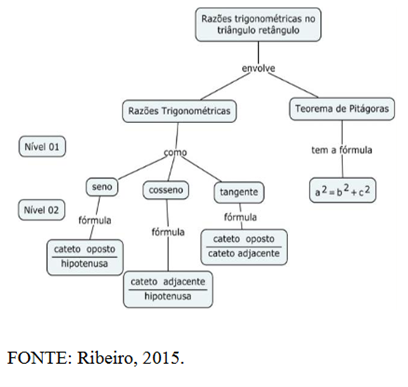
\includegraphics[width=\linewidth]{superficie-professor1}
  \end{figure}
  \columnbreak

  Segundo \citet{moreira2011} não existe um mapa “certo” ou “errado”, pois os mapas conceituais construídos pelos alunos têm componentes idiossincráticos. Porém apresentam evidências do nível conceitual do aluno, bem como sua evolução ao compararmos um mapa inicial, isto é, para detectar conhecimentos prévios, com um mapa final, construído após a organização de conceitos apresentados.

  Os mapas conceituais podem ser construídos no papel, quando a atividade for individual ou em pequenos grupos, na lousa para uma atividade em grande grupo (por exemplo, ao final de uma socialização onde é necessário fazer uma formalização das discussões) ou ainda com o auxílio do software \textit{Cmap Tools 6.04} (\url{https://cmaptools.br.uptodown.com/windows}). Deixaremos nas referências alguns vídeos e textos que abordam os mapas conceituais como ferramentas essenciais no ensino, caso o colega tenha interesse.

  \subsection{Sugestões de metodologias}

  Conforme \citet{BNCC2019}, resolver e elaborar problemas amplia e aprofunda o significado dado à resolução de problemas: a elaboração pressupõe que os estudantes investiguem outros problemas que envolvem os conceitos tratados; sua finalidade é também promover a reflexão e o questionamento sobre o que ocorreria se algum dado fosse alterado ou se alguma condição fosse acrescentada ou retirada.

  Para \citet{dambrosio1989}',' a típica aula de matemática na educação básica, ainda nos dias de hoje, consiste em professores como papel principal, na exposição de conteúdos por eles julgados importantes, enquanto que os alunos tentam resolver exercícios de aplicação, que nada mais são do que uma repetição na aplicação de um modelo de solução apresentado pelo professor.

  Já \citet{skovsmose2014} afirma que quando trabalhamos com questões previamente formuladas, as atividades em sala de aula podem ser reduzidas ao certo ou errado. Desta forma o autor propõe os cenários para investigação, que são situações sobre a qual as atividades de ensino e aprendizagem acontecem.

  O autor ainda destaca que ao criar um cenário para investigação o professor deve pensar a respeito da matemática que pode ser explorada por meio dele. Porém estas propostas de cenários para investigação devem ser significativas para os alunos.
  \columnbreak
  \begin{quote}
  A experiência da significação depende de os alunos trazerem suas intencionalidades para as atividades de aprendizagem. Investigar e explorar são atos conscientes, eles não acontecem como atividades forçadas. \citep[p. 60]{skovsmose2014}.
  \end{quote}
  Desta forma, o que sugerimos ao colega professor é uma reflexão sobre suas concepções quanto ao ensino de Matemática. Os cenários para investigação propostos neste capítulo devem ser analisados e adaptados (se assim forem necessários) a realidade e contexto que sua sala de aula necessita.

  Entendemos que esse não seja um processo rápido, porém não impossível. A competência na qual está inserida a habilidade deste capítulo pressupõe utilizar estratégias, conceitos, definições e procedimentos matemáticos para interpretar, construir modelos e resolver problemas em diversos contextos, analisando a plausibilidade dos resultados e a adequação das soluções propostas, de modo a construir argumentação consistente \citep[p. 535]{BNCC2019}

  Segundo \citet{barbosa2001}, a modelagem é um ambiente de aprendizagem no qual os alunos são convidados a indagar e/ou investigar, por meio da matemática, situações oriundas de outras áreas da realidade. O autor ainda propõe, a partir de sua pesquisa em nível nacional e internacional, três casos para a modelagem, mas reitera que em todos eles o professor é mediador do processo de ensino e aprendizagem.

  \begin{enumerate}[label=\titem{\arabic*)}]
  \item Caso 1. O professor apresenta a descrição de uma situação-problema, com as informações necessárias à sua resolução e o problema formulado, cabendo aos alunos o processo de resolução. 
  \item Caso 2. O professor traz para a sala um problema de outra área diferente da Matemática, cabendo aos alunos a coleta das informações necessárias à sua resolução. 
  \item Caso 3. A partir de temas não-matemáticos, os alunos formulam e resolvem problemas. Eles também são responsáveis pela coleta de informações e simplificação das situações-problema. 
  \end{enumerate}

  Estamos apenas instigando uma reflexão e pesquisa por parte de você, professor! Deixaremos mais referências para sua análise e reflexão.
\end{apresentacao}

\begin{paginatexto}{O que é área?}
\subsection{Objetivos Gerais}

\begin{itemize}
\item Reconhecer o conceito de área de superfície por meio da caracterização da região no plano ou no espaço delimitado por curvas (poligonais ou não) fechadas.
\item Avaliar abordagens distintas e aplicação de técnicas diversificadas para o cálculo de áreas de superfícies irregulares.
\item Aplicar o conhecimento de que a área de uma figura plana fechada e limitada pode ser medida usando uma unidade fixada (quadrado ou triângulo, por exemplo) de comparação e de contagem, buscando implementar um processo de medição, e aplicar métodos algébricos para as fórmulas que advêm das medidas das unidades.
\end{itemize}

\textbf{Quantidade de aulas previstas para a primeira seção}: 6 horas/aula.
Enriquecimento da discussão:

Conforme \citet{BNCC2019} os estudantes do Ensino Médio devem construir e ampliar a noção de medida, pelo estudo de diferentes grandezas, a fim de obter expressões para o cálculo da medida da área de superfícies planas e da medida do volume de alguns sólidos geométricos. O documento ainda destaca a necessidade de construir uma visão integrada da Matemática, aplicada à realidade, em diferentes contextos.

\begin{quote}
Consequentemente, quando a realidade é a referência, é preciso levar em conta as vivências cotidianas dos estudantes do Ensino Médio – impactados de diferentes maneiras pelos avanços tecnológicos, pelas exigências do mercado de trabalho, pelos projetos de bem viver dos seus povos, pela potencialidade das mídias sociais, entre outros \citep[p. 528]{BNCC2019}
\end{quote}

Desse modo, a Matemática deve se responsabilizar a 

\begin{quote}
Desenvolver habilidades relativas aos processos de investigação, de construção de modelos e de resolução de problemas. Para tanto, eles devem mobilizar seu modo próprio de raciocinar, representar, comunicar, argumentar e, com base em discussões e validações conjuntas, aprender conceitos e desenvolver representações e procedimentos cada vez mais sofisticados.\citep[p. 529]{BNCC2019}.
\end{quote}

Conforme \citet{santos2014} para auxiliar os alunos a formularem o conceito de área, é necessário que o professor tenha domínio dos conceitos de superfície, área e medida da área. Neste capítulo, trabalhamos “superfície” como um conceito geométrico, a “área associada a uma porção da superfície” como uma grandeza que pode ser medida, e que a “medida da área de uma porção de superfície” pode ser expressa em números, assim como em fórmulas algébricas. Segundo \citet{lima2013}, o ato de medir uma grandeza é uma comparação com uma grandeza fixada de mesma natureza, usada como “unidade de referência”, quando essa comparação produz um resultado numérico tanto pela contagem desta unidade dentro da grandeza inicial, como pelo valor numérico resultante das operações com a “medida numérica da unidade de referência”.

De acordo com \citet{lima2013}, 

\begin{quote}
Para encontrar a área de uma figura F, devemos comparar sua superfície (a porção do plano que ele ocupa) com a de uma outra figura tomada como unidade. O resultado dessa comparação será um número que deverá exprimir quantas vezes a figura F contém a unidade de área \citep[p. 92]{lima2013}.
\end{quote}

Para figuras planas, adotamos, em geral, como unidade de área o quadrado cujo lado mede uma unidade de comprimento, que chamamos de \textit{quadrado unitário}. Assim, se o lado do quadrado for de $1$cm, a unidade de área será chamada de \textit{centímetro quadrado} e representada por $1$\textit{cm}$^2$. Desse modo, para cada unidade de comprimento existe uma unidade de área correspondente. Todavia, para determinar a área de uma figura qualquer, tudo o que podemos conhecer sobre sua área são aproximações. Como podemos comparar a superfície de uma figura qualquer com o quadrado unitário? Quanto mais preciso forem nossos métodos mais precisas serão nossas aproximações.

Para \citet{BNCC2019} desenvolver a competência de raciocinar requer a interação dos alunos com colegas e professores, investigação, explicação e justificativa das soluções apresentadas para os problemas, com ênfase nos processos de argumentação matemática. A competência de representar está associada ao uso dos registros de representação e das diferentes linguagens que, muitas vezes, é necessário para a compreensão, a resolução e a comunicação de resultados de uma atividade. 

Ao resolverem os problemas matemáticos, os estudantes precisam apresentar e justificar seus resultados, interpretar os resultados dos colegas e interagir com eles. Seu desenvolvimento pressupõe também a formulação e a testagem de conjecturas, com a apresentação de justificativas, o que compete a comunicação e argumentação.

Para que essas competências sejam alcançadas o professor deve submeter seus alunos a situações de aprendizagem que exijam do aluno elaboração de hipóteses e a construção de modelos matemáticos para situações da realidade.

\begin{quote}
O professor de Matemática deve compreender que é um mediador do processo de construção do conhecimento matemático e, para isso, sua prática, deve oportunizar aos estudantes exercitarem a capacidade de buscar soluções para os problemas, haja visto que o ritual de apresentação do conceito, das propriedades, da fórmula, do algoritmo e da série de exercícios de aplicação com modelos repetitivos, não está sendo eficaz \citep[p. 235]{santos2014}.
\end{quote}

Dessa forma, o que estamos propondo para essa primeira seção é um momento de interação onde as competências raciocinar, representar, comunicar e argumentar estejam evidentes. Após a verificação dos conhecimentos prévios de seus alunos, sugerimos organizá-los em grupos (de no máximo 4 alunos) para a realização das atividades propostas.  Ao verificar os conceitos que eles apresentam é a oportunidade para averiguar as dificuldades ainda apresentadas, corrigir os erros evidentes e conduzir os alunos a construir o conceito adequado.

Sugerimos que seja respeitado o tempo necessário para a discussão, argumentação, raciocínio e representação das atividades em cada grupo. Após a resolução é muito significativo a socialização e a discussão das ideias em grande grupo. Lembre-se que você, professor, deve ser o mediador dessa socialização para que ao final das atividades seja possível apresentar o conceito de área, e assim sirva de ancoragem para novos conhecimentos.

Sugerimos para essa seção atividades onde a área de uma figura exprime quantas vezes essa figura contém a unidade de área. O que pretendemos aqui é mediar o conceito de área com as generalizações, isto é, as fórmulas que serão apresentadas na próxima seção. 

\textbf{Organização da turma}: Grupos de até 4 alunos. Socialização das respostas com todos os alunos.

\textbf{Sobre as atividades da primeira seção}: Para as atividades \textit{“Parque Estadual do Turvo, Potencial Híbrido de uma planta e Poluição por derramamento de petróleo”}, apresentamos o conceito de área partindo de três abordagens diferentes: a diferença entre área e perímetro, a unidade de área e área por aproximações. Também destacamos a oportunidade de utilizar aplicativos de medição já na atividade inicial, para que o professor tenha a oportunidade de verificar os problemas conceituais da turma. Observe que esse é um objetivo de ensino, não de aprendizagem. Uma sugestão é concentrar os seus esforços na interação. Deixe os grupos discutirem e utilize esta oportunidade para verificar os conhecimentos prévios da turma. Também anote informações importantes para serem discutidas na socialização em grande grupo. Para a primeira atividade, escolhemos um parque importante no RS, mas sugerimos ao professor que além desta atividade valorize também parques e reservas provenientes de sua região. Para as atividades pensamos em contextualizações com outras áreas do conhecimento, para que os alunos percebam a importância do conceito de área em outros contextos. 
\end{paginatexto}



\cleardoublepage
\def\currentcolor{session1}
\begin{objectives}{O Parque Estadual do Turvo}
{
Entender o conceito de área como um espaço delimitado por curvas e saber diferenciá-lo de perímetro.
}{1}{1}
\end{objectives}
\begin{sugestions}{O Parque Estadual do Turvo}{
A atividade objetiva verificar os conteúdos prévios dos alunos quanto a perímetro e área. Observe o que seus alunos pensam sobre perímetro e sobre área, o que significam e se sabem diferenciá-los. Sugerimos ao professor promover uma discussão e socializa-la em grupo, afim de verificar se ainda existe alguma dificuldade nos conceitos.

Para esta atividade pensamos em oportunizar a utilização de recursos tecnológicos para resolvê-la. Segue um roteiro, caso o professor não esteja familiarizado com o aplicativo. Escolhemos um aplicativo simples que pode ser acessível em qualquer local.



\begin{enumerate}
\item Acesse \url{https://www.google.com/maps/d/} 
\item Clique em Mapa sem Título

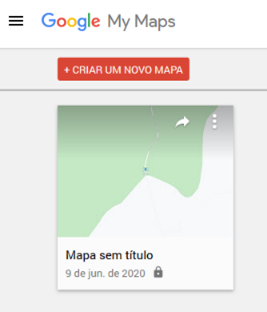
\includegraphics[width=.3\textwidth]{superficie-professor2}
\item Na barra de busca escreva "Parque Estadual do Turvo"
\item No menu "Mapa Básico", mude para Satélite.


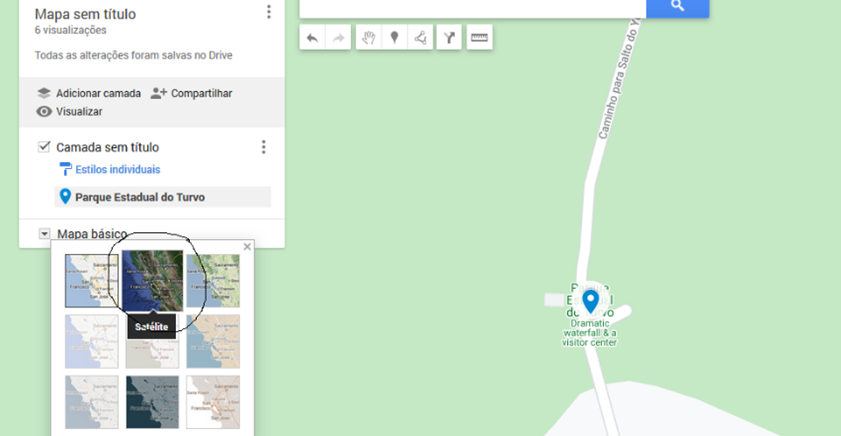
\includegraphics[width=.75\linewidth]{superficie-professor3}


\item Diminua a imagem
\begin{figure}[H]
\centering

\resizebox{.9\textwidth}{!}{
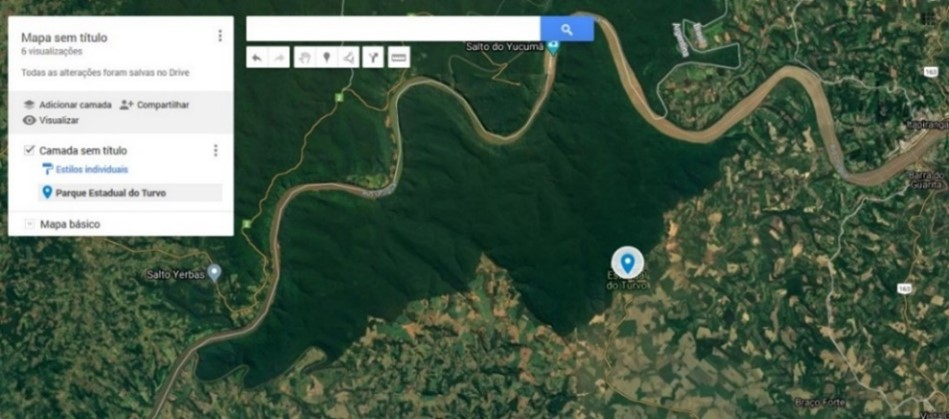
\includegraphics[height=100bp]{superficie-professor4}
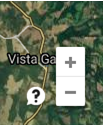
\includegraphics[height=100bp]{superficie-professor5}
}
\end{figure}

\item Clique em medir distâncias e áreas.

\item Clique onde você deseja iniciar sua medição.
\item Clique em cada canto ou curva de uma linha ou forma.
\item Quando você terminar de desenhar, clique duas vezes ou feche a forma em outro ponto.
\item Você verá a distância (e a área, se for uma forma) destacada em azul no mapa. Distâncias e áreas são baseadas na sua escala e no seu país.

\centering
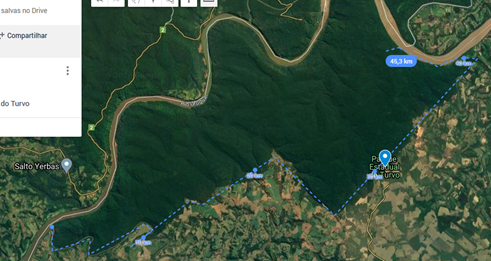
\includegraphics[width=.6\textwidth]{superficie-professor6}

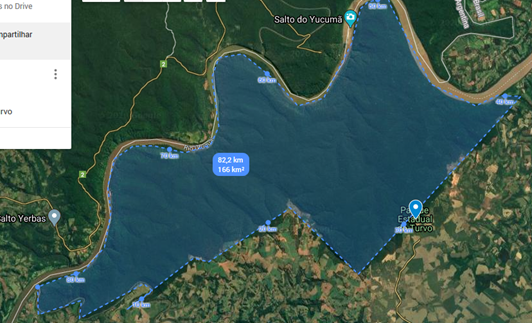
\includegraphics[width=.6\textwidth]{superficie-professor7}

\end{enumerate}
}{0}{9}
\end{sugestions}
\clearmargin
\begin{answer}{O Parque Estadual do Turvo}
{
  \begin{enumerate}
  \item Sim, é possível. Para determinar o perímetro devemos demarcar o contorno da figura e fazer a medição e a região delimitada por este contorno é o que chamamos de área.
  \item 
  \begin{itemize}
  \item Perímetro: aproximadamente $82{,}2$km.
  \item Área: aproximadamente $166$km$^2$.
  \end{itemize}
  
  \end{enumerate}
}{1}
\end{answer}

\begin{objectives}{Outras experiências}
{
  Entender as relações existentes entre área e perímetro, checando que figuras com áreas diferentes podem ter perímetros iguais.
}{1}{0}
\end{objectives}
\begin{sugestions}{Outras experiências}
{
  Na figura temos apenas um exemplo. Após a resolução do exercício fazer trocas das folhas entre os grupos para a socialização e discussão posterior.

  \textbf{Material necessário}: folhas A4 e tesouras
}{1}{2}
\end{sugestions}
\begin{answer}{Outras experiências}
{
  O perímetro será sempre o mesmo, o que muda é a área da região.
}{1}
\end{answer}
\begin{objectives}{Potencial híbrido de uma planta}
{
  Aplicar o conceito de unidade de área usando uma unidade fixada (quadrado ou triângulo, por exemplo), buscando implementar um processo de medição para o cálculo de áreas de superfícies irregulares.
}{1}{0}
\end{objectives}
\begin{sugestions}{}
{
  Esta atividade exige o conhecimento prévio de proporcionalidade, pois quanto maior a área da folha maior será sua taxa de transpiração. Nos vegetais, a quantidade de folhas e a superfície foliar são fatores que determinam maior ou menor taxa de transpiração. Isso porque na estrutura de uma folha existem células estomáticas responsáveis pelas trocas gasosas. A taxa de transpiração é medida como a quantidade de água perdida por m² e por minuto e existe um experimento para calcular. Você pode conseguir mais informações sobre o experimento em (\url{http://www.phschool.com/science/biology_place/labbench/lab9/analysis1.html}). 

  No entanto, a atividade vai apresentar apenas como você deve estimar a área da superfície foliar da planta. Acreditamos ser uma oportunidade para trabalhar no contexto da Biologia ou de forma interdisciplinar. Caso o colega opte por fazer a atividade apenas contextualizando, é muito importante discutir com os alunos a respeitos dos conceitos de Biologia, porém deve destacar que a atividade trata apenas de uma técnina  para estimar a área da superfície foliar da planta. Esta atividade é muito importante, pois mais adiante no capítulo trabalharemos a relação entre o aumento da medida dos lados do quadrado referência produzir ou não um aumento proporcional da medida da área da figura. 

  \textbf{Material necessário}: Folhas de plantas, papel quadriculado.

}{1}{1}
\end{sugestions}
\begin{answer}{Potencial híbrido de uma planta}
{
  \begin{enumerate}
  \item A resposta depende das folhas que os alunos encontrarem.

  \item Quanto maior a folha, maior sua taxa de transpiração.
  \end{enumerate}
}{1}
\end{answer}
\explore{O que é área?}

Saber resolver problemas utilizando o conceito de área, nos mais diferentes contextos, dentro da Matemática ou com outras áreas do conhecimento é a objetivo deste capítulo. Contextos significativos, não somente no contexto escolar, mas também em questões ligadas a comunidade e ao mundo do trabalho. Ao final desta unidade espera-se que você, estudante, seja capaz de, por exemplo,  calcular a quantidade de tinta necessária para pintar uma casa, não desperdiçar tecido para fabricar uma peça de roupa, determinar a área de terrenos, calcular a quantidade de lajotas para cobrir pisos e paredes, determinar a área de faces de objetos, entre tantos outros problemas ligados ao conceito de área.

\begin{task}{O Parque Estadual do Turvo}

\begin{multicols}{2}

O Parque Estadual do Turvo, criado em de 11 de março de 1947, como Reserva Florestal, foi uma das primeiras unidades de conservação instituídas no Rio Grande do Sul em 1954, sendo a maior área protegida de proteção integral do Estado.

\begin{figure}[H]
\centering

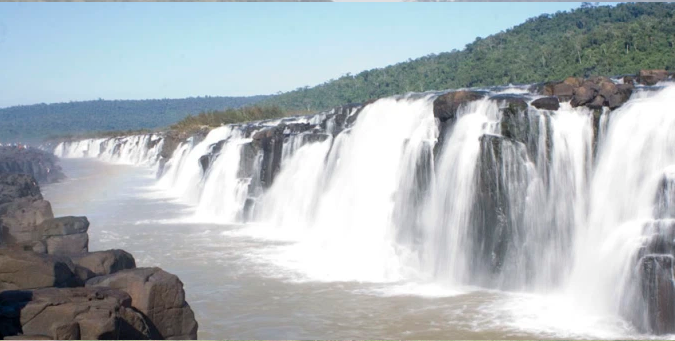
\includegraphics[width=200bp]{superficie1}

\caption{Salto do Yucumã, Parque Estadual do Turvo. Foto: D. Meller}
\end{figure}

\end{multicols}

É o último refúgio para animais como a onça-pintada, a anta e o gavião-real (harpia) no Rio Grande do Sul. Por tais atributos é considerado por muitos ambientalistas como a área mais importante para conservação da fauna gaúcha ameaçada de extinção. O principal atrativo turístico do parque é o Salto do Yucumã, a maior queda d’água longitudinal do mundo, com 1800 metros de extensão.

Situa-se no município de Derrubadas, no extremo Noroeste do Rio Grande do Sul, Brasil. Através do Rio Uruguai faz fronteira com a província argentina de Misiones e divisa com o estado brasileiro de Santa Catarina (\url{https://parquedoturvo.wordpress.com}).

\begin{figure}[H]
\centering

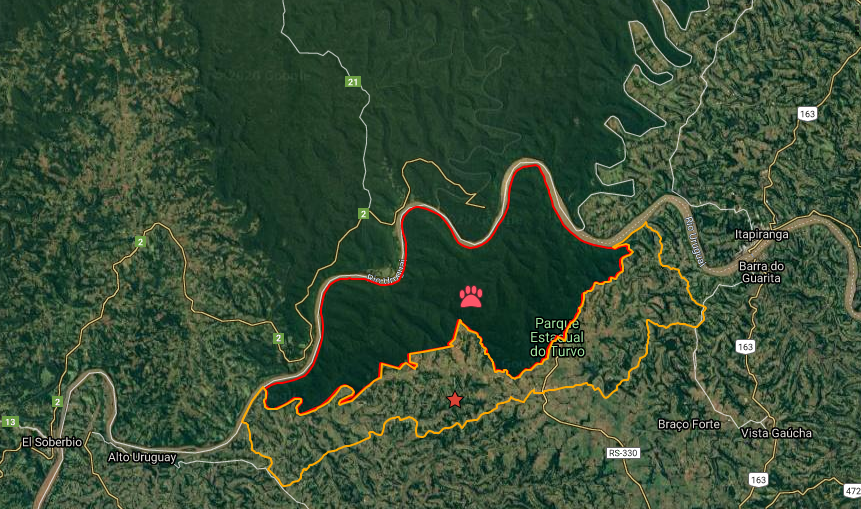
\includegraphics[width=290bp]{superficie2}

\end{figure}

\begin{enumerate}
  \item É possível calcular a área e o perímetro do parque? Discuta com seu grupo e descreva um método para obter a área e o perímetro da região anterior.
  \item Com o auxílio de \textit{Google My Maps}, calcule a área e o perímetro aproximado do Parque Estadual do Turvo.
\end{enumerate}
\end{task}

\begin{task}{Outras experiências}
Uma folha retangular de papel foi cortada de um vértice ao vértice oposto, formando dois pedaços. Qual pedaço te perímetro maior?
\begin{figure}[H]
\centering

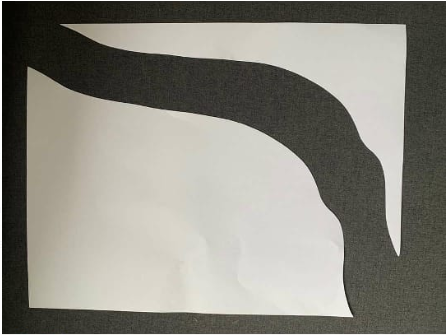
\includegraphics[width=200bp]{superficie3}

\end{figure}
\end{task}

\begin{task}{Potencial híbrido de uma planta}
(Atividade adaptada de \href{http://www.phschool.com/science/biology_place/labbench/lab9/calcsurf.html}{Pearson Prentice Hall})

\begin{wrapfigure}{r}{.5\textwidth}
\centering
  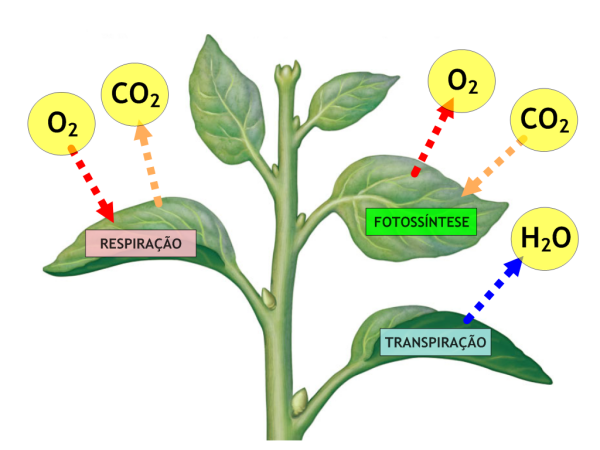
\includegraphics[width=200bp]{superficie4.png}
  \caption{Fonte: \href{https://www.estudokids.com.br/respiracao-e-transpiracao-dos-vegetais/)}{Estudo Kids}}
\end{wrapfigure}  
A respiração é essencial para a sobrevivência de todos os animais e também dos vegetais. Quando os seres vivos respiram, o oxigênio que está presente no ar é inspirado e o gás carbônico é expirado. Todos os seres vivos passam por esse processo, inclusive as plantas. A transpiração dos vegetais é um processo que ocorre quando a planta absorve água em excesso. 

Assim como na respiração, a principal parte do vegetal que é responsável por realizar a transpiração é a folha. Com o intenso calor e tempo seco de alguns lugares, os vegetais passaram a evoluir obtendo, desta forma, mecanismos reguladores quanto à absorção, retenção e perda de água. O excesso de água desses vegetais é liberado pelas folhas para o meio ambiente através de pequenas gotinhas de água que se transformam em vapor. Quando as temperaturas estão muito elevadas em certo período do dia, a planta fecha seus estômatos para não perder muita água para o meio ambiente e consequentemente ficar desidratada.

É importante saber que a quantidade de folhas e a superfície foliar são fatores determinantes para a maior ou menor taxa de transpiração, isso acontece devido às células estomáticas. A taxa de transpiração é medida como a quantidade de água perdida por m$^2$ e por minuto. Para chegar à taxa de transpiração, portanto, você deve calcular a área de superfície foliar de cada planta: 

\begin{figure}[H]
\centering

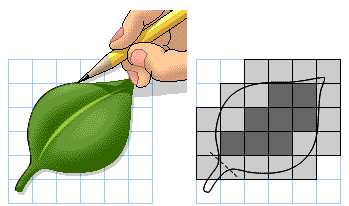
\includegraphics[width=200bp]{superficie5}

\end{figure}

\begin{itemize}
  \item Coloque as folhas a serem medidas em uma grade de $1$cm e trace seus contornos.
  \item Conte o número de centímetros quadrados. Estime a área dos quadrados parciais (conte um quadrado parcial se estiver pelo menos metade coberto pela folha; não conte quadrados parciais com menos do que meio coberto).
  \item Não inclua a área da haste (pecíolo) em seus cálculos.
\end{itemize}

\begin{enumerate}
  \item Consiga algumas folhas de tamanhos diferentes e calcule a sua área.
  \item Como a água evapora através dos muitos estômatos (são estruturas da epiderme da planta localizadas nas folhas e responsáveis pelas trocas gasosas e pela transpiração) na superfície da folha, a taxa de transpiração está diretamente relacionada à área da superfície. O que significa isso?
\end{enumerate}
\end{task}
\clearpage
\begin{knowledge}
O cálculo da área de sua superfície ocorre de uma maneira especial. Observe a figura a seguir, ela representa a superfície de uma região plana irregular: 

\begin{figure}[H]
\centering

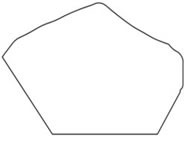
\includegraphics[width=150bp]{superficie6}

Figura A
\end{figure}

Para calcularmos a sua área uma opção é transpor a figura sobre um papel quadriculado, da seguinte forma: 

\begin{figure}[H]
\centering

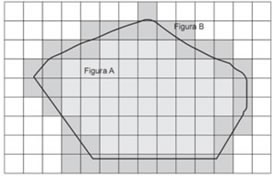
\includegraphics[width=175bp]{superficie7}

Figura B
\end{figure}

Realizada essa ação, é preciso contar o número de quadrados inteiros que preenchem o interior da figura. A área por falta da figura é de $43$ quadrados (figura A).

Observe que se, contar o número de quadrados inteiros que cobrem toda a figura, a área por excesso da região é de $80$ quadrados (figura B). 

Para determinarmos a área aproximada da figura, que está entre $43$ e $80$, utilizamos uma média aritmética da quantidade de quadriculados encontrados: 
\begin{equation*}
A=\frac{43+90}{2}=61{,}5.
\end{equation*}

A unidade de área utilizada será a da figura no tamanho original. Nesse caso, a área da figura dada se encontra em m$^2$, então, cada quadriculado representa $1$m$^2$. Portanto, a área da região irregular é de aproximadamente $61{,}5$m$^2$.

Fonte: \href{https://brasilescola.uol.com.br/matematica/calculo-de-areas-especiais.htm}{Brasil Escola}
\end{knowledge}

\clearpage

\begin{objectives}{Poluição por derramento de petróleo}
{
  Aplicar uma técnica para o cálculo de área de uma figura plana fechada e limitada a partir da unidade fixada, em situações do cotidiano.
}{1}{1}
\end{objectives}
\begin{sugestions}{Poluição por derramento de petróleo}
{
  Sugerimos ao professor discutir com os alunos que a foto da atividade não dá ideia de verdadeira grandeza, implicando que os quadrados na superfície do mar são diferentes nas regiões da figura, porém que para facilitar os cálculos consideraremos todos com o mesmo tamanho.
}{1}{1}
\end{sugestions}
\begin{answer}{Poluição por derramento de petróleo}
{
  \begin{enumerate}
  \item 
  \begin{itemize}
  \item Área por falta = $49$
  \item Área por excesso = $70$
  \item Área = $\dfrac{49+70}{2}=59{,}5$
  \end{itemize}
  \item Cada quadrado equivale a $100$km$^2$, assim, $59{,}5\times100=5950$km$^2$.
  \end{enumerate}
}{1}
\end{answer}

\begin{task}{Poluição por derramamento de petróleo}
(Atividade adaptada de \href{https://www.tecnologiae.com.br/poluicao-derramamento-petroleo-quais-consequencias/}{Tecnologia É})

Nosso planeta, a Terra, tem grandes reservas de petróleo e gás presas nas profundezas de sua superfície. Ocasionalmente, essas reservas desenvolvem rachaduras e parte do petróleo ou gás vaza. Nos últimos anos, a questão dos derramamentos de óleo e seus efeitos assumiu grande importância. Isso ocorre porque quando ocorre um derramamento de óleo há uma infinidade de problemas para o ambiente e para nós. Como derramamento de óleo, ele flutua na água e impede a passagem da luz solar. A substância brilhante que você vê, por vezes, na camada superior da água não é nada, mas é petróleo que torna difícil para as plantas e animais marinhos para sobreviverem. Limpar o derramamento de óleo não é tarefa fácil. Vários fatores precisam ser considerados antes de realizar as operações. Alguns deles sendo quantidade de óleo derramado, temperatura da água, tipo de praias e muito mais.

\begin{figure}[H]
\centering

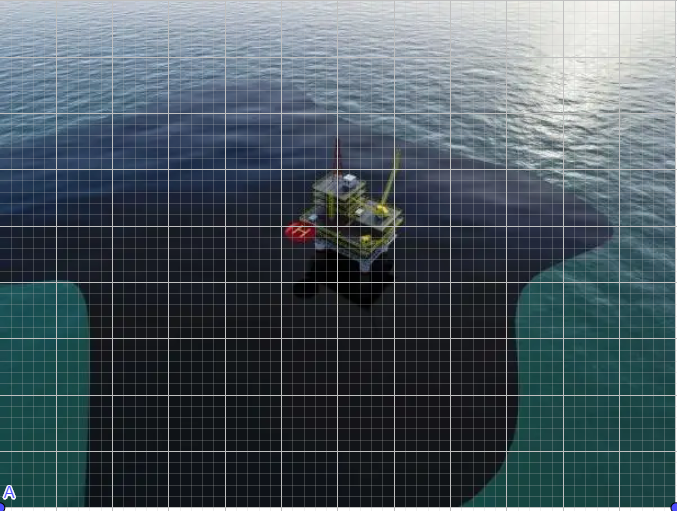
\includegraphics[width=325bp]{superficie8}


\caption{Foto: Times Now}
\end{figure}

\begin{enumerate}
  \item Calcule a área aproximada da mancha apresentada na foto acima
  \item Utilizando a escala do mapa, determine a área em km$^2$.
\end{enumerate}

\end{task}

\arrange{Conceituando área}

Para \textit{medir} uma grandeza devemos compará-la com uma outra de mesma espécie tomando-a como unidade. Assim, quando vamos medir uma porção do plano ocupada por uma figura, esta medida é a sua área.

\begin{quote}
Para encontrar a área de uma figura F, devemos comparar sua superfície (a porção do plano que ele ocupa) com a de uma outra figura tomada como unidade. O resultado dessa comparação será um número que deverá exprimir quantas vezes a figura F contém a unidade de área \citep[p. 92]{lima2013}.
\end{quote}

A área de uma figura exprime quantas vezes essa figura contém uma \textit{unidade de área}. Observe a figura a seguir. Consideramos a unidade de área como cada triângulo.
\begin{multicols}{2}
\begin{figure}[H]
\centering

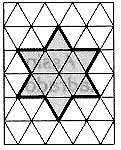
\includegraphics[width=100bp]{superficie9}
\end{figure}
\columnbreak

\null\vfill
\begin{figure}[H]
\centering

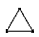
\includegraphics[width=25bp]{superficie10}
$1$ unidade de área

\medskip

Área de figura: 12 unidades de área
\end{figure}
\vfill\null
\end{multicols}

Em geral, adotamos como \textit{unidade de área} o quadrado cujo lado mede uma unidade de comprimento. Sendo assim, para cada unidade de comprimento existe uma unidade de área correspondente.

\begin{figure}[H]
\centering

\begin{tikzpicture}
\draw[fill=\currentcolor!80] (0,0) rectangle (1,1);
\draw [->] (0.5,0.5) -- (2.5,0.5) node [right] {$1$ unidade de área};
\node [below] at (.5,0) {$1$ unidade de comprimento};
\draw [very thick] (0,0) -- (1,0);
\end{tikzpicture}
\end{figure}

Assim, por exemplo, ao considerarmos um quadrado de lado $1$cm, a unidade de área será chamada de \textit{centímetro quadrado} (cm$^2$). Logo,



\begin{figure}[H]
\centering

\begin{tikzpicture}
\tikzstyle{quad}=[minimum width=1cm, minimum height=1cm, draw, node distance=1cm];

\node [fill=\currentcolor!80, quad] (a) {\small$1$cm$^2$};

\begin{scope}[xshift=4cm]
\node [fill=\currentcolor!80, quad] (a) {};
\node (b) [right of=a, quad] {};
\node (c) [below of=b, quad] {};
\node (d) [above of=b, quad] {};
\node (e) [right of=b, quad] {};

\node [below of=c] {Área da figura = $4$cm$^2$};
\end{scope}
\end{tikzpicture}
\end{figure}

Mas como poderemos comparar a superfície de uma figura qualquer com a unidade de área? Para figuras com formatos mais irregulares poderemos determinar a sua área por aproximações. Quanto mais preciso forem nossos métodos, melhor será a nossa aproximação.

\begin{paginatexto}{Área de figuras planas}

\subsection{Objetivos Gerais}
\begin{itemize}
\item Entender o processo de dedução da fórmula para o cálculo de área de figuras.
\item Entender o processo de aplicação de fórmulas, as relações matemáticas existentes e sua formalização em problemas reais.
\item Entender a relação que existe entre área delimitada por uma figura poligonal fechada no plano com a área de uma figura semelhante a ela por um fator de proporcionalidade $k$. 
\end{itemize}

\textbf{Quantidade de aulas previstas para a seção}: 8 horas/aula.

\textbf{Organização da turma}: Grupos de até 4 alunos. Socialização das respostas com todos os alunos.

\subsection{Enriquecimento da discussão}

Colega professor, não esqueça que deduzir expressões de cálculo para aplicá-la em situações reais é previsto pela habilidade que norteia este capítulo. O que estamos sugerindo é uma nova abordagem de ensino. Como você já observou anteriormente, é muito importante que seus alunos saibam conceituar área, mas também saber calcular áreas de polígonos e círculos são básicos para o desenvolvimento dessa habilidade.

Para isso, objetiva-se nessa seção entender o processo de dedução de uma fórmula para calcular área de figuras, tais como os quadriláteros, os triângulos, círculos e figuras regulares como o hexágono, por exemplo. Conforme \citet{BNCC2019} a Geometria não pode ficar reduzida a mera aplicação de fórmulas de cálculo de área ou de volume.

Ainda no Ensino Fundamental – Anos Finais, a expectativa é que os alunos devem determinar expressões de cálculo de áreas de quadriláteros, triângulos e círculos, mas assumindo que no Ensino Médio deve haver a consolidação, a ampliação e o aprofundamento das aprendizagens essenciais devemos apresentá-la de forma mais integrada. Assim, sugerimos explorar a relação de dependência entre duas grandezas na busca do desenvolvimento do pensamento proporcional.

\begin{quote}
  Isso pode ser feito pela exploração de situações que oportunizem a representação, em um sistema de coordenadas cartesianas, da variação de grandezas, além da análise e caracterização do comportamento dessa variação (diretamente proporcional, inversamente proporcional ou não proporcional) \citep[p. 528]{BNCC2019}.
 \end{quote}

Dessa forma, \citet{BNCC2019} ainda propõe que os estudantes utilizem tecnologias. Entendemos nessa seção uma oportunidade para a utilização de softwares, em particular o GeoGebra (\url{https://www.geogebra.org/}). O GeoGebra é um software livre, de matemática dinâmica, vindo ao encontro de novas estratégias de ensino e aprendizagem, permitindo a professores e alunos a possibilidade de explorar, conjecturar e investigar na construção do conhecimento matemático.

\subsection{Sugestões de materiais e metodologias}

Nesta seção gostaríamos de sugerir aos colegas alguns materiais disponíveis na internet. Para a construção e análise de fórmulas apresentados nesta seção, sugerimos o software GeoGebra. Não somente nesta seção, mas em todo o capítulo você pode explorar atividades no GeoGebra. Este software também pode ser acessado pelo celular, sendo assim mais uma opção, caso o laboratório de informática de sua escola não disponha de máquinas muito eficientes.

Na figura a seguir, temos um exemplo de atividade retirado do site \url{https://www.geogebra.org/} . Sugerimos aos colegas explorarem este site, pois somente você poderá saber quais atividades podem ser significativas para a realidade de seus alunos. 

\begin{figure}[H]
\centering

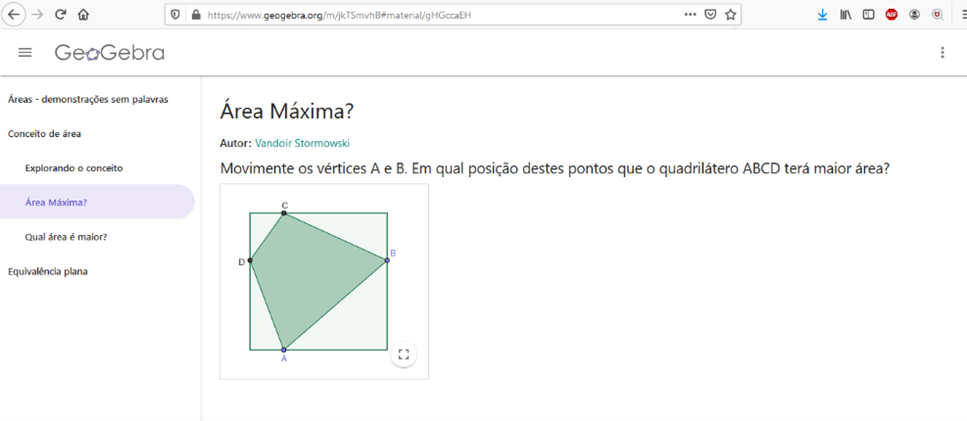
\includegraphics[width=.925\linewidth]{superficie-professor8}
\caption{Exemplo de atividade no GeoGebra. Fonte: \url{https://bit.ly/3lIvfhj}}
\end{figure}

Para o professor que não tem muita experiência em utilizar o software ou talvez ainda não o conheça, existe um curso de capacitação de GeoGebra, a fim de abordar seus aspectos técnicos e disponibiliza materiais e recursos para fomentar reflexões sobre seu uso em situações de ensino e aprendizagem (ver \cite{ogeogebra2020}).

Caso você tenha dúvidas sobre os conceitos envolvidos no capítulo sugerimos o livro \textit{“Temas e Problemas Elementares}” da Coleção PROFMAT, assim como “\textit{A Matemática do Ensino Médio – Volume 2}” da Coleção do Professor de Matemática – SBM (ver Referências Bibliográficas).

Também gostaríamos de sugerir o Programa de Aperfeiçoamento de Professores de Matemática do Ensino Médio – PAPMEM \citep{impa2020}, que consiste em um treinamento gratuito para professores de matemática de todo o Brasil. É realizado desde 1990 abordando assuntos relativos ao Ensino Médio. O programa é realizado durante uma semana em tempo integral, das 9 às 17 horas, de modo independente nos meses de janeiro e julho, durante o recesso escolar. 

\textbf{Sobre as atividades da seção} Algumas atividades foram adaptadas do site \url{https://m3.ime.unicamp.br/} . Você pode encontrar maiores detalhes nos links citados na atividade. 

\end{paginatexto}

\def\currentcolor{session1}
\begin{objectives}{A reforma da sala}
{
  Aplicar o conceito de área e outras grandezas (comprimento) em situações do cotidiano
}{1}{1}
\end{objectives}
\begin{sugestions}{A reforma da sala}
{
  Você pode apresentar o exercício com materiais e os preços da realidade de sua comunidade escolar e depois propor a resolução desta atividade. Também é uma oportunidade para observar os conhecimentos prévios dos alunos quanto as figuras planas por eles conhecidas e suas respectivas fórmulas para cálculo de área. A atividade exige conhecimento prévio de transformações de medidas e porcentagem.

  \textbf{Material necessário}: Caderno, calculadora.

}{1}{1}
\end{sugestions}
\begin{answer}{A reforma da sala}
{
\begin{enumerate}
  \item 
  \textbf{Para o piso}: Área do chão = $5{,}3 \text{m} \times 4{,}5 \text{m} = 23{,}85$m². Cada pacote tem $2{,}25$m², então $23{,}85/2,25=10{,}6$, isto é, $11$ pacotes. Comprando $10\%$ deste total a mais temos $11 \times 1{,}1= 12{,}1$, isto é, $13$ pacotes.

  \textbf{Para o Painel 3D}: Área da parede = $5{,}3 \text{m} \times 2{,}7 \text{m} = 14{,}31$m². As placas são quadradas de $0{,}5$m de lado, logo a área de cada uma é $0{,}5 \text{m} \times 0{,}5 \text{m} = 0{,}25$m². Então $14{,}31/0,25 = 57{,}24$ placas, isto é, $58$ placas. Comprando $10\%$ a mais temos $58 \times 1{,}1= 63{,}8$, isto é, $64$ placas. Logo, $64 \text{ placas} \times 0{,}25 \text{m²} = 16 $m².

  \textbf{Para o Rodapé}: Perímetro da sala = $5{,}3 \times 2 + 4,50 \times 2 = 19{,}6$m. Desconsiderando a largura da porta, temos $19{,}6 \text{m} - 0{,}8 \text{m} = 18{,}8$m. Cada peça tem $2100 \text{mm} = 2{,}1$m, logo $18{,}8 / 2{,}1= 8{,}8$, isto é, $9$ peças. Comprando $10\%$ a mais temos $9 \times 1{,}1 = 9{,}9$, logo $10$ peças.

  \textbf{Tinta}: Área das Paredes = $5{,}3 \times 2{,}7 \times 2 + 4{,}5 \times 2{,}7 = 40{,}77$ m². Área da porta = $0{,}8 \text{m} \times 2{,}2 \text{m} = 1{,}76$m². Área do teto = $5{,}3 \text{m} \times 4{,}5 \text{m} = 23{,}85$m². Assim, a área total $=$ área das paredes $+$ área do teto $-$ área da porta $=$ $40{,}77+23{,}85 - 1{,}76 =62,86$ (m²). Utilizando a dica para o consumo de galões (latas), temos Consumo $=$ $(62{,}86 \times 2) /10=12{,}57$, logo $13$ galões. 

  \textbf{Para a moldura}: Perímetro da sala = $5{,}3 \times 2 + 4{,}50 \times 2 = 19{,}6$m. Cada peça tem $1$m, então $19{,}6$, logo $20$ peças. Comprando $10\%$ a mais temos $20 \times 1{,}1 = 22$ peças.
\end{enumerate}

}{1}
\end{answer}
\begin{answer}{A reforma da sala}
{
  \begin{enumerate}\setcounter{enumi}{1}
  \item 
  \adjustbox{valign=t}
  {
  \begin{tabular}{|>{\centering}d{.2\linewidth}|>{\centering}d{.2\linewidth}|c|c|}
  \hline
  \tcolor{ Material} & \tcolor{Preço Unitário} & \tcolor{Quantidade} & \tcolor{Preço Final} \\
  \hline
  Piso & R\$ $67{,}00$ a caixa & $13$ & $13\times67=871{,}00$ \\
  \hline
  Placas de Gesso 3D & R\$ $49{,}90$ por m$^2$ & $16$ & $16\times49{,}9=798{,}40$\\
  \hline
  Rodapé & R\$ $9{,}38$ por m & $10\times 2{,}1=21$m & $21\times9{,}38=196{,}98$\\
  \hline
  Tinta & R\$ $149{,}90$ a lata ($18\ell$) & $13$ & $22\times 5{,}5=121{,}00$\\
  \hline
  Moldura de Gesso & R\$ $5{,}50$ a peça & $22$ & R\$ $3938{,}08$\\
  \hline
  \textbf{Total} & --- & --- & \\
  \hline
  \end{tabular}
  }

  \end{enumerate}
}{0}
\end{answer}
\explore{Área de figuras planas}

\begin{task}{a reforma da sala}

Marcelo pretende investir na reforma da sala de seu apartamento. Vai trocar o pixo, colocar gesso no teto, criar um painel de gesso e pintar. Para isso está pesquisando os materiais necessários.

\begin{table}[H]
\centering
\setlength\tabcolsep{3pt}
\begin{tabular}{|l|ll|}
\hline
Piso laminado & Régua: $8\text{mm}\times187\text{mm}\times 1350$mm & Caixa: $16{,}65\text{kg}/2{,}2552\text{m}^2$ \\

Placas de gesso 3D (pintado) & Tamanho: $0{,}50\text{m}\times0{,}50\text{m}$ & \\

Tinta & Lata de $18\ell$ & Rendimento: $10\text{m}^2$ por $\ell$ \\

Rodapé de MDF & \multicolumn{2}{l|}{Tamanho: $80\text{mm}\times15\text{mm}\times2100\text{m}$} \\

Moldura de Gesso & \multicolumn{2}{l|}{Medidas: $3\text{cm}\times3\text{cm}$, $1$ metro de comprimento} \\
\hline
\end{tabular}
\end{table}



Sabendo que a sala tem dimensões $5{,}30\text{m}\times4{,}50\text{m}\times2{,}70\text{m}$, uma porta de $2{,}20\text{m}\times0{,}80\text{m}$ e a janela ocupa toda uma parede da sala (ver figura). O painel de gesso 3D vai ficar na parede oposta à porta da sala.

\begin{figure}[H]
\centering

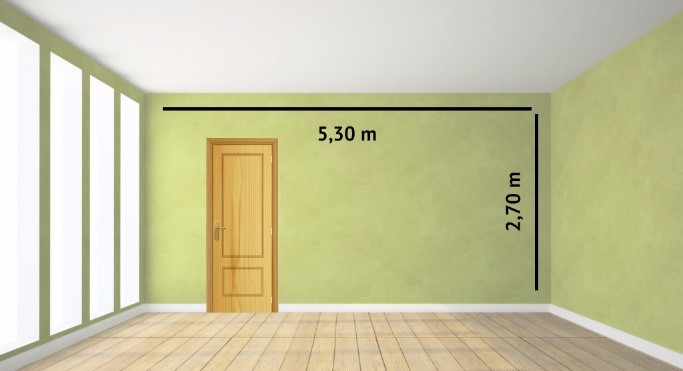
\includegraphics[width=200bp]{superficie11}\hspace{1cm}
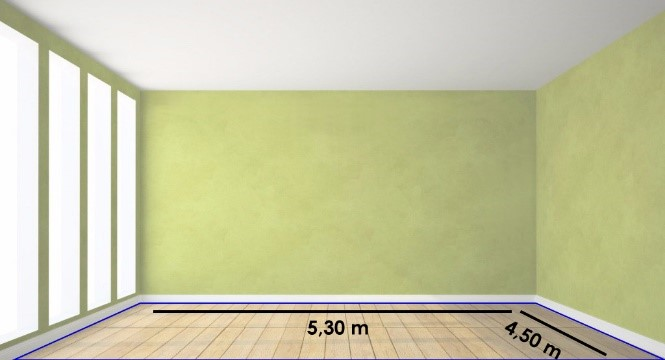
\includegraphics[width=200bp]{superficie12}

\caption{Fonte: \href{https://blog.sincenet.com.br/como-calcular/}{Sincenet}}
\end{figure}

\begin{enumerate}
  \item Calcule a quantidade mínima necessária de cada material, sbendo que Marcelo vai adquirir $10\%$ a mais por segurança e vai dar duas demãos.

  \textbf{Dica}: Consumo de galões = metragem quadrada $\times$ número de demãos $/$ rendimento por lata (informado pelo fabricante).

  \item Calcule o custo total dos materiais.

  \begin{table}[H]
  \centering
  
  \begin{tabular}{|c|c|c|c|}
  \hline
  \tcolor{Material} & \tcolor{Preço Unitário} & \tcolor{Quantidade} & \tcolor{Preço Final} \\
  \hline
  Piso & R\$ $67{,}00$ a caixa & & \\
  \hline
  Placas de Gesso 3D & R\$ $49{,}90$ por m$^2$ & & \\
  \hline
  Rodapé & R\$ $9{,}38$ por m & & \\
  \hline
  Tinta & R\$ $149{,}90$ a lata ($18\ell$) & & \\
  \hline
  Moldura de Gesso & R\$ $5{,}50$ a peça & & \\
  \hline
  \textbf{Total} & --- & & \\
  \hline
  \end{tabular}
  \end{table}
\end{enumerate}

\end{task}
\clearpage
\begin{objectives}{Empacotamento de latas}
{
  Reconhecer a área e comprimento de setores circulares através de um problema de otimização.
}{1}{2}
\end{objectives}
\begin{sugestions}{Empacotamento de latas}
{
  Neste experimento, os alunos tentarão descobrir qual deve ser a disposição de uma quantidade fixa de latas, de forma que o custo para as embalar seja o menor possível. Peça para que cada aluno traga de casa 4 latas de alumínio de mesmo tamanho e forma. Os alunos deverão estar atentos a dois problemas: o primeiro é encontrar a disposição que minimiza o custo para embalar uma quantidade fixa de latas; o segundo, no final do experimento, é encontrar, dentre todas as possíveis escolhas, aquela que minimiza o custo de embalagem por lata. A seguir, peça para que os grupos escolham uma quantidade entre 3 e 12 latas para formar suas embalagens. 

  Nesta etapa, o importante é obter uma grande variedade entre os grupos para o fechamento do experimento. É necessário, portanto, que cada grupo escolha quantidades diferentes de latas. Padronize o tipo de lata que os alunos devem trazer, pois isso é essencial para o experimento. O problema deste experimento considera apenas o custo. A embalagem de cada caixa deve cobrir as latas por completo e estar ajustada aos seus contornos. Note que o custo será o menor possível quando a área superficial da embalagem em uma dada disposição das latas também for a menor possível. 

  Este problema tem o contexto muito interessante e importante de forma que os alunos podem perceber a importância de saber calcular a área de figuras planas. Neste experimento, os alunos irão solucionar um problema de otimização que envolve a embalagem de latas: qual é a disposição de uma quantidade fixa de latas que fornece o menor custo possível de embalagem? É claro que as latinhas devem encostar umas às outras e não podem ser amassadas. Em termos formais, os círculos não se sobrepõem, mas não deve haver nem um círculo isolado (exceto o caso trivial de uma única latinha). Além do mais o material de empacotamento adere ao contorno de parte de uma latinha, mas ao passar de uma latinha para a outra o material vai sair pela tangente de um círculo e chegar ao outro círculo também em tangente. Estas condições matemáticas são satisfeitas aproximadamente no experimento prático. Mais informações sobre o experimento, sobre conceitos matemáticos envolvidos e as possíveis disposições das latas você consegue em \url{https://m3.ime.unicamp.br/recursos/1009}. 

  \textbf{Material necessário}: Latas de alumínio, Calculadora, Régua, Folha de caderno, Compasso.
}{0}{9}
\end{sugestions}
\begin{answer}{Empacotamento de latas}
{
  \begin{enumerate}
  \item Vamos resolver para o caso de 6 latas. Para outra quantidade de latas e outras disposições, os cálculos devem seguir um raciocínio análogo

  \begin{figure}[H]
  \centering
  
  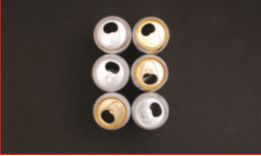
\includegraphics[width=.4\linewidth]{superficie-professor9}\hspace{1em}
  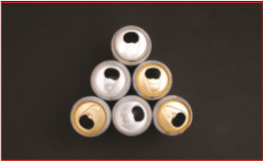
\includegraphics[width=.4\linewidth]{superficie-professor10}

  Disposição 1 \hspace{.25\linewidth} Disposição 2

  \vspace{1em}
  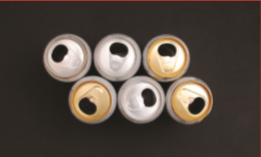
\includegraphics[width=.4\linewidth]{superficie-professor11}

  Disposição 3
  \end{figure}
  \item
    \begin{enumerate}
    \item Quantidade de latas: 6
    \item Altura ($h$): $12{,}5$cm
    \item Raio ($r$): $3{,}5$cm
    \item\adjustbox{valign=t}
    {
    \begin{tabular}{|c|c|}
    \hline
    \tcolor{Disposição} & \tcolor{Área (cm$^2$)} \\
    \hline
    1 & $1366{,}67$* \\
    \hline
    2 & $1340{,}60$* \\
    \hline
    3 & $1340{,}60$* \\
    \hline
    \end{tabular}

    *Valores aproximados
    }
    \end{enumerate}
    \item Disposição 1 ou 2.
    \item $1340{,}6/6=223{,}4$cm²
  \end{enumerate}
}{1}
\end{answer}
\clearmargin
\begin{objectives}{Retângulos crescentes}
{
  Entender a relação que existe entre área delimitada por uma figura poligonal fechada no plano com a área de uma figura semelhante a ela por um fator de proporcionalidade k. 
}{1}{1}
\end{objectives}
\begin{sugestions}{Retângulos crescentes}
{
  Induza os alunos a serem investigativos, utilizando números decimais e não somente inteiros. Na Parte 2 da atividade explore outras figuras, tais como poligonal fechada, figuras não regulares, o círculo. Lembre-se que desta forma a atividade se torna mais complexa e empolgante, porque os alunos estão usando suas ideias e pensamentos.

  \textbf{Material necessário}: Papel quadriculado ou Geogebra. A atividade pode ser explorada em \url{https://www.geogebra.org/m/v4csscej} 

}{1}{1}
\end{sugestions}
\begin{answer}{Retângulos crescentes}
{
  Espera-se que os alunos compreendam a razão de semelhança entre as figuras e que, sendo k a razão de semelhança então a razão entre suas áreas será k². Segue um exemplo:

  \begin{figure}[H]
  \centering
  
  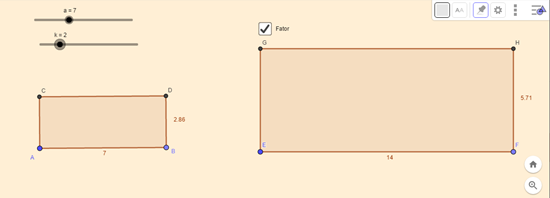
\includegraphics[width=\linewidth]{superficie-professor12}
  \end{figure}

  \begin{align*}
  A_1=7\times2{,}86=20{,}02 \quad\quad\quad A_2  =14\times 5{,}71=79{,}94\\
  \end{align*}
  $$\frac{A_2}{A_1}=4=2^2=k^2$$
}{1}
\end{answer}

\begin{task}{empacotamento de latas}
(Atividade adaptada. Fonte: \href{https://m3.ime.unicamp.br/recursos/1009}{IME - Unicamp})

A sociedade moderna já se acostumou com bebidas e alimentos em latas de formato cilíndrico de tamanho apropriado para o uso individual. As indústrias então têm o desafio de transportar grandes quantidades de latas. Para facilitar o transporte é comum pequenos fardos com várias latas e estas são transportadas em caminhões e navios. 

\begin{figure}[H]
\centering

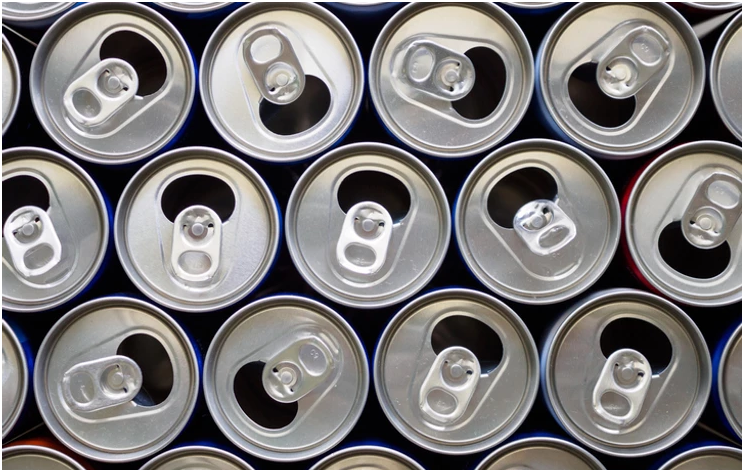
\includegraphics[width=300bp]{superficie13}

\caption{Fonte: \href{https://www.guaranamineiro.com.br/post/latas-de-alumínio-brasil-é-o-maior-reciclador-do-mundo}{Guaraná Mineiro}}
\end{figure}

A matemática tem ferramentas interessantes para otimizar o empacotamento de objetos. Qual será a melhor disposição de forma que o custo para embalar as latas seja o menor possível?

\begin{enumerate}
  \item Escolham três disposições que vocês acham que oferecem os menores custos de embalagem. Registrem no caderno as três disposições escolhidas e numere-as de 1 a 3.
  \item Meça a altura ($h$) e o raio ($r$) da lata. Calcule a área da embalagem utilizada em cada uma das situações.
    \begin{enumerate}
    \item Quantidade de latas:
    \item Altura ($h$):
    \item Raio ($r$):
    \item\adjustbox{valign=t}
    {
    \begin{tabular}{|c|c|}
    \hline
    \tcolor{Disposição} & \tcolor{Área (cm$^2$)} \\
    \hline
    1 & \\
    \hline
    2 & \\
    \hline
    3 & \\
    \hline
    \end{tabular}
    }
    \end{enumerate}
  \item Qual das disposiões oferece a embalagem de menor custo?
  \item Com a embalagem de menor custo, calcule o custo de embalagem por lata $A/Q$
\end{enumerate}

\end{task}
\begin{reflection}
Por que a melhor disposição encontrada não é aquela que as empresas usam para embalar as latas?
\end{reflection}

\begin{task}{Retângulos crescentes}
(Atividade adaptada do livro Mentalidades Matemáticas)

\textbf{Parte 1}

Considere um retângulo com $20\text{cm}^2$ de área.

\begin{enumerate}
  \item Qual poderia ser seu comprimento e sua largura? Cite ao menos 5 combinações diferentes.
  \item Agora, amplie cada cada retângulo por um fator escalar $2$.
  \item Liste as dimensões de seus retângulos ampliados e descubra suas áreas. O que você nota?
  \item Desta vez, pense em retângulos ampliados e descubra suas áreas. O que você nota?
  \item Desta vez, pense em retângulos de áreas diferentes e os amplie por um fator escalar $2$.
  \item Você sabe explicar o que está acontecendo?
  \item O que acontece com a área de um retângulo se você o amplia por um fator escalar de 3? E se esse escalar for um número fracionário?
  \item O que acontece com a área de um retêngulo se você o amplia por um fator escalar $k$? Explique e justifique suas conclusões.
\end{enumerate}

\textbf{Parte 2}

Refaça a atividade anterior para outras formas planas, além de reângulos. Explique e justifique suas conclusões.
\end{task}

\arrange{Área de figuras planas}

Como já definimos anteriormente, para medir uma porção do plano ocupada por uma figura $F$, devemos compará-la com a unidade de área, e assim o resultado será um número que exprime quantas vezes a figura $F$ contém a unidade de área.

Desse modo, nessa seção vamos organizar essa ideia com um significado mais preciso. Para isso, vamos lembrar das figuras planas mais conhecidas e suas respectivas fórmulas para determinar a sua área.


\subsection{Área do quadrado e do retângulo}

O quadrado é o quadrilátero que tem os 4 lados iguais e os 4 ângulos retos. Se a medida do do lado de um quadrado é $a$, um número real qualquer (inteiro, fracionário ou irracional), sua área é igual a $a^2$, e expressa pela fórmula 
\begin{equation*}
A=a^2.
\end{equation*}

\begin{figure}[H]
\centering

  \begin{tikzpicture}
  \draw [fill=\currentcolor!80] (0,0) rectangle (5,5);
  \draw [\currentcolor!80!black] (0,0) grid (5,5);

  \node [above, overlay] at (2.5,5) {$5$cm};
  \node [right, overlay] at (5,2.5) {$5$cm};
  \end{tikzpicture}

$a=5$cm \hspace{2cm} $A=25$cm$^2$

\caption{Versão interativa: \url{https://www.geogebra.org/m/hsXHDRX7\#material/xpcbYhKT}}
\end{figure}

O retângulo é o quadrilátero que tem os 4 ângulos retos. Se os lados de um retângulo $R$ têm como medidas dois números reais $a$ e $b$, a área de um retângulo é o produto das medidas de seus lados, e expressa pela fórmula 
\begin{equation*}
A=a\times b.
\end{equation*}

\begin{figure}[H]
\centering

  \begin{tikzpicture}
  \draw [fill=\currentcolor!80] (0,0) rectangle (6,4);
  \draw [\currentcolor!80!black] (0,0) grid (6,4);

  \node [above, overlay] at (3,4) {$6$cm};
  \node [right, overlay] at (6,2) {$4$cm};
  \end{tikzpicture}

$a=6$cm,\quad $b=4$cm \hspace{2cm} $A=4\times6=24$cm$^2$

\caption{Versão interativa: \url{https://www.geogebra.org/m/JJDxunvT}}
\end{figure}

\clearpage

\subsection{Área de um paralelogramo}

Conhecida a área de um retângulo, podemos calcular a área de um paralelogramo. O Paralelogramo é um quadrlátero no qual os lados opostos são paralelos. Quando se toma um lado do paralelogramos como base, chama-se altura $a$ um segmento perpendicular que liga a base ao lado oposto (ou aos seu prolongamento).

A área de um paralelogramo é, portanto, o produto da base pela altura, e expressa pela fórmula 
\begin{equation*}
A=b\times h.
\end{equation*}

\begin{figure}[H]
\centering

\begin{tikzpicture}[scale=.9]

\draw [fill=\currentcolor!80] (.5,.5) -- (2.5,4) -- (7.5,4) -- (5.5,.5) -- cycle;
\draw [step=.5, gray!90] (0,0) grid (8,4.5);
\draw (.5,.5) -- (2.5,4) -- (7.5,4) -- (5.5,.5) -- cycle;

\begin{scope}[xshift=8.25cm]

\draw [fill=\currentcolor!80] (.5,.5) -- (2.5,4) -- (7.5,4) -- (5.5,.5) -- cycle;

\begin{scope}
\clip (4,.5) rectangle (7.5,4);
\draw [fill=session2!80] (.5,.5) -- (2.5,4) -- (7.5,4) -- (5.5,.5) -- cycle;
\draw [thick] (4,.5) -- (4,4) node [pos=.5, right] {$h$};

\draw (4,.5) rectangle (4.5,1);
\draw (4,4) rectangle (4.5,3.5);
\end{scope}
\draw [step=.5, gray!80] (0,0) grid (8,4.5);
\draw (.5,.5) -- (2.5,4) -- (7.5,4) -- (5.5,.5) -- cycle;

\end{scope}

\end{tikzpicture}

\end{figure}
\begin{figure}[H]
\centering

\begin{tikzpicture}[scale=.9]

\draw [fill=\currentcolor!80] (.5,.5) rectangle (5.5,4);
\draw [thick] (2,.5) -- (4,4); 
\draw (.5,.5) rectangle (1,1);
\draw (.5,4) rectangle (1,3.5);

\node [right] at (.5,2) {$h$};

\begin{scope}
\clip (2,.5) -- (4,4) -- (.5,4) -- (.5,.5) -- cycle;
\draw [fill=session2!80] (.5,.5) rectangle (7.5,4);
\end{scope}
\draw [step=.5, gray!90] (-1,0) grid (7,4.5);
\draw (.5,.5) rectangle (5.5,4);

\end{tikzpicture}

\caption{Versão interativa: \url{https://www.geogebra.org/m/R42DVZ8K\#material/D8rjsGzF}}
\end{figure}

\subsection{Área de um triângulo}

Da área de um paralelogramo, passamos imediatamente par a área de um triângulo, pois todo triângulo é a metade de um paralelogramo.

Assim, a área de um triângulo é, portanto, a metade do produto da base pela altura, e expressa pela fórmula 
\begin{equation*}
A=\frac{b\times h}{2}.
\end{equation*}

\begin{figure}[H]
\centering


\begin{tikzpicture}[scale=.9]

\draw [fill=\currentcolor!80] (.5,.5) -- (2.5,4) -- (5.5,.5) -- cycle;

\end{tikzpicture}\quad
\begin{tikzpicture}[scale=.9]

\draw [fill=\currentcolor!80] (.5,.5) -- (2.5,4) -- (7.5,4) -- (5.5,.5) -- cycle;
\draw (2.5,4) -- (5.5,.5);

\end{tikzpicture}


\caption{Versão interativa: \url{https://www.geogebra.org/m/R42DVZ8K\#material/uKQKXvu3}}
\end{figure}

\textbf{Obs.}: Observe que em um triângulo temos 3 opções para base $b$ e, portanto, três opções para a altura $h$. Em qualquer uma das opções sempre teremos o dobro da área do triângulo. Dessa forma, a área de um triângulo não se altera quando sua base permanece fixa e o vértice oposto percorre uma reta paralela à base.

\begin{figure}[H]
\centering

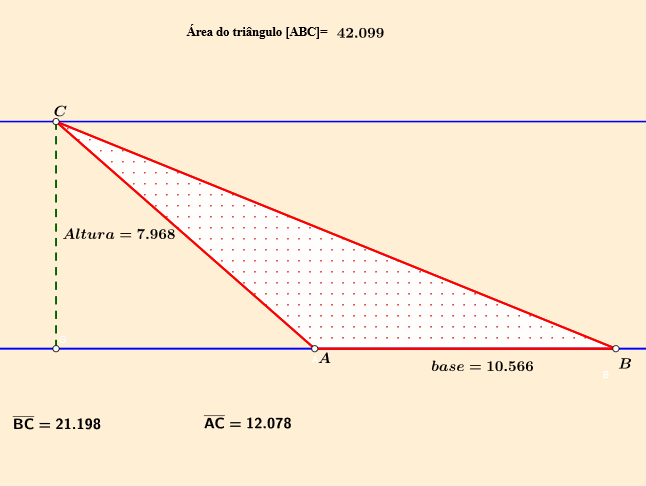
\includegraphics[height=135bp]{superficie21}\hspace{1em}
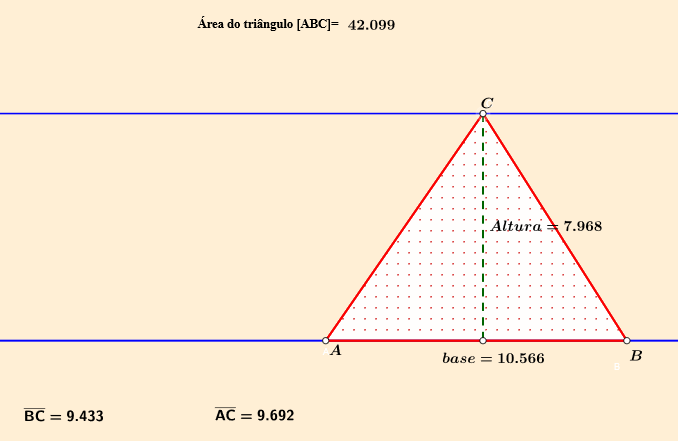
\includegraphics[height=135bp]{superficie22}

\caption{Versão interativa: \url{https://www.geogebra.org/m/uq5VxUcW}}
\end{figure}

\subsection{ Área de um trapézio}

Chamamos de base média de um trapézio ao segmento de reta que une os pontos médios dos lados não paralelos. Sua medida é a média aritmética das medidas das bases.

A área do trapézio é o produto da base média pela altura, expressa pela fórmula 
\begin{equation*}
A=\frac{(b+b)\times h}{2}.
\end{equation*}

\begin{figure}[H]
\centering

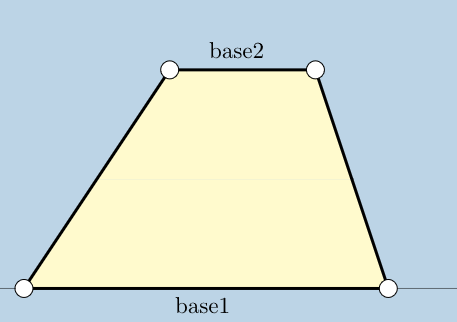
\includegraphics[height=85bp]{superficie23}\hspace{.5em}
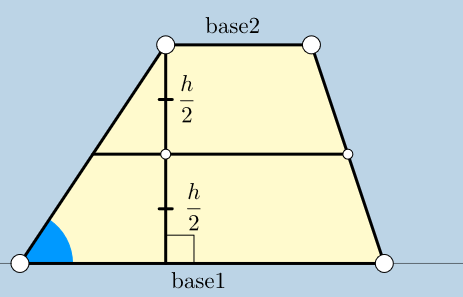
\includegraphics[height=85bp]{superficie24}\hspace{.5em}
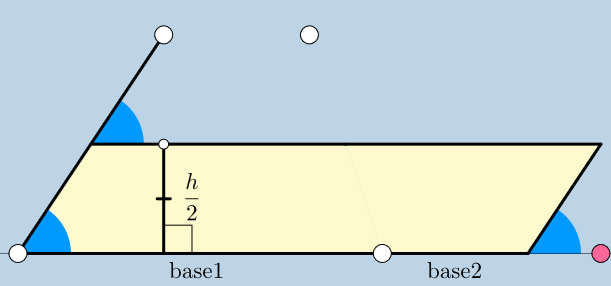
\includegraphics[height=85bp]{superficie25}

\caption{Versão interativa: \url{https://www.geogebra.org/m/R42DVZ8K\#material/rktj8gqv}}
\end{figure}

\subsection{ Área de um losango}

Um losango é um quadrilátero que tem os lados com medidas iguais. A área do losango é a metade do produto das medidas de suas diagonais, expressa pela fórmula  
\begin{equation*}
A=\frac{D\times d}{2}.
\end{equation*}

\begin{figure}[H]
\centering

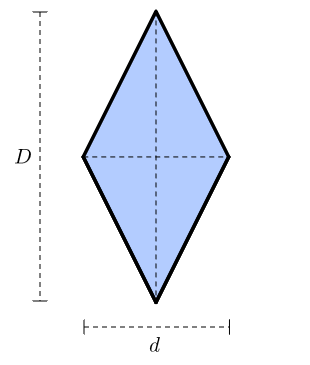
\includegraphics[height=135bp]{superficie26}\hspace{.5em}
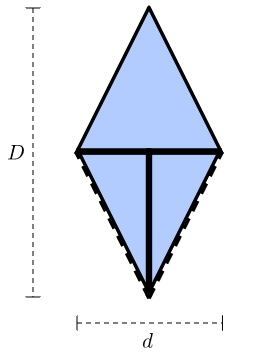
\includegraphics[height=135bp]{superficie27}\hspace{.5em}
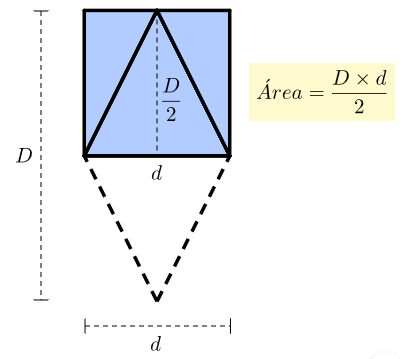
\includegraphics[height=135bp]{superficie28}

\caption{Versão interativa: \url{https://www.geogebra.org/m/fUEGv6D6}}
\end{figure}

Para um polígono qualquer, para calcular a sua área, podemos subdividi-lo em figuras tais como triângulos, quadriláteros ou outra qualquer cuja área sabemos calcular. Desta forma, a área do polígono procurado será a soma das áreas das figuras em que o decompusemos.

\subsection{ Área de um hexágono regular}

Para o cálculo da área de qualquer polígono regular basta calcularmos a área de um dos triângulos isósceles a partir do centro do polígono e multiplicá-la pelo número de lados do polígono.

\begin{multicols}{2}
\centering
Área do triângulo equilátero: 
\begin{equation*}
A=\frac{l^2\sqrt{3}}{4}.
\end{equation*}

Área do triângulo equilátero: 
\begin{equation*}
A=6\times\frac{l^2\sqrt{3}}{4}
\end{equation*}
\end{multicols}

\begin{figure}[H]
\centering

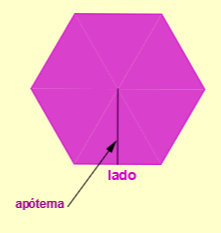
\includegraphics[height=85bp]{superficie29}\hspace{1em}
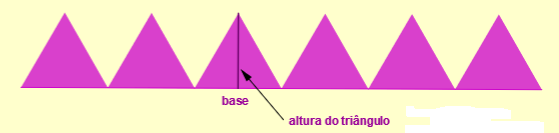
\includegraphics[height=85bp]{superficie30}

\caption{Versão interativa: \url{https://www.geogebra.org/m/RgAY5xdQ}}
\end{figure}

\clearpage
\subsection{Área do círculo}

A área de um círculo de raio $r$ é uma função desse raio. Então a área de um círculo de raio $r$ é expressa pela fórmula
\begin{equation*}
A=\pi r^2.
\end{equation*}

\begin{figure}[H]
\centering

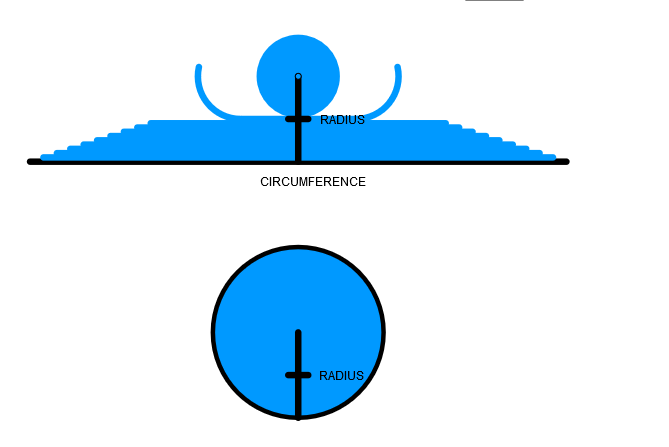
\includegraphics[height=125bp]{superficie31}\hspace{1em}
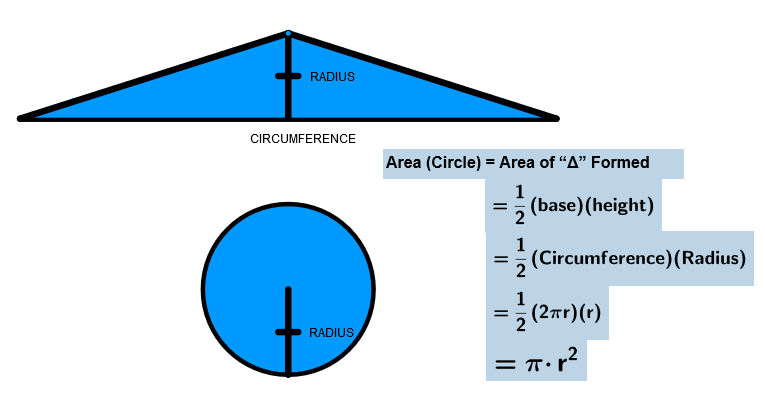
\includegraphics[height=125bp]{superficie32}

\caption{Versão interativa: \url{https://www.geogebra.org/m/R42DVZ8K\#material/Ga3e6tfV}}
\end{figure}
\clearpage

\def\currentcolor{session2}
\begin{objectives}{Reforma da piscina}
{
  Aplicar relações entre área e outras grandezas (comprimento) em situações diversas. 
}{1}{1}
\end{objectives}
\begin{sugestions}{Reforma da piscina}
{
  A atividade tem caráter de aplicação dos conceitos construídos no Explorando, em particular o cálculo da área de quadriláteros
}{1}{1}
\end{sugestions}
\begin{answer}{Reforma da piscina}
{
  \begin{itemize}
  \item Área $= 10\times6+10\times 1{,}6\times+6\times1{,}6\times2=111{,}24$m²
  \item Área do ladrilho $=0{,}20\text{m}\times0{,}20\text{m}=0{,}04$m². Assim, $111{,}2/0{,}04=2780$ ladrilhos
  \end{itemize}
}{1}
\end{answer}
\clearpage
\begin{objectives}{Quadra de basquete 3$\times$3}
{
  \begin{itemize}
  \item Aplicar relações entre área e outras grandezas(comprimento) em situações diversas. 
  \item Reconhecer as diferentes figuras planas e saber calcular a área correspondente.
  \end{itemize}
}{1}{1}
\end{objectives}
\begin{sugestions}{Quadra de basquete 3$\times$3}
{
  A atividade tem caráter de aplicação dos conceitos construídos no Explorando, em particular o cálculo da área de figuras planas. As informações em vermelho no desenho são as medidas das figuras.
}{1}{1}
\end{sugestions}
\clearmargin
\begin{answer}{Quadra de basquete 3$\times$3}
{
\begin{itemize}
\item   Área Vermelha $=$ área do retângulo $= 5,8 \text{m}\times4,88 \text{m} = 28,304$m²

\item Área Branco $=\dfrac{\text{área do círculo}}{2}=\dfrac{3{,}14\cdot(1{,}85)^2}{2}=5{,}37$m² (observe que $3{,}70$ é o diâmetro)

\item Área Azul $= \dfrac{\text{área do círculo}}{2}+\text{área do retângulo}-(\text{área vermelha}+\text{área branca})$

\item Área Azul $=\dfrac{3{,}14\cdot(6{,}3)^2}{2}+12{,}6\cdot2{,}87-(28{,}304+5{,}37)=64{,}8$m²
 
\item $\text{Área Verde}=\text{área do retângulo}-\\\bigg(\dfrac{\text{área do círculo}}{2}+\text{área do retângulo}\bigg)$

\item Área Verde = $15\times11-\bigg(\dfrac{3{,}14\cdot(6{,}3)^2}{2}+12{,}6\cdot2{,}87\bigg)=66{,}52$m²
\end{itemize}

Como vão passar duas demãos na quadra, temos:
\begin{itemize}[left=0pt]\setlength{\columnsep}{2cm}
\begin{multicols}{2}
\item Vermelha: $2\times28{,}304=56{,}608$m²
\item Azul: $2\times64{,}8=129{,}6$m²
\item Branco: $2\times5{,}37=10{,}74$m²
\item Verde: $2\times66{,}52=133,04$m²
\end{multicols}
\end{itemize}

Dessa forma, sabendo que cada lata rende $70$m², os amigos devem comprar 1 lata de tinta vermelha, 1 lata de tinta branca, 2 latas de tinta azul e 2 latas de tinta verde.

Assim, $6\times$R\$ $68{,}60$= R\$ $411{,}60$. Logo, os amigos ainda não têm dinheiro suficiente.

}{1}
\end{answer}
\begin{objectives}{A praça}
{
\begin{itemize}
\item Aplicar relações entre área e outras grandezas (comprimento) em situações diversas. 
\item Reconhecer as diferentes figuras planas e saber calcular a área correspondente.
\end{itemize}
}{1}{2}
\end{objectives}
\begin{sugestions}{A praça}
{
  A atividade tem caráter de aplicação dos conceitos construídos no Explorando, em particular o cálculo da área de figuras planas. Para este exercício você deve revisar sobre Função Quadrática.
}{1}{2}
\end{sugestions}
\begin{answer}{A praça}
{
\begin{enumerate}
\item A área de cada canteiro de pedra para $x=2$ vale $\frac{2\times8}{2}$. Assim, a área do canteiro de grama é  $100-4\times8=68$m². 
  
\item A área de cada canteiro triangular é dada pela expressão $A=\frac{x(10-x)}{2}$. Assim, a área do canteiro de grama é dada por $A=\text{área do quadrado}-4\times\text{área do triângulo}$
\begin{equation*}
A= 100-4\times\frac{x(10-x)}{2}=2x^2-20x+100
\end{equation*}
\item  O custo será $C=4\cdot\text{área de grama} + 3\times\text{Área de pedra}$
Sabe-se que o custo da área de grama será $4\cdot(2x^2-20x+100)$  e o custo da área de um canteiro é $3\cdot\frac{x(10-x)}{2}$. Assim, o custo total será dado pela expressão  
\begin{align*}
C&=4\cdot(2x^2-20x+100)+4\cdot3\cdot\frac{x(10-x)}{2}\\
C&=2x^2-20x+400
\end{align*}
Lembrando que o valor extremo de uma função quadrática, dá-se para $y=\frac{-\Delta}{4a}$, ou seja, a ordenada do vértice.  Neste caso, precisamos determinar o custo mínimo, logo, 
\begin{equation*}
y=\frac{-[(-20)^2-4\cdot2\cdot400)]}{4\cdot}=\frac{2800}{8}=350. 
\end{equation*}
Ou ainda, R\$ $350{,}00$.
\end{enumerate}
}{1}
\end{answer}
\begin{objectives}{Arcos de circunferência}
{
  Entender o processo de aplicação de fórmulas, as relações matemáticas existentes e sua formalização em problemas reais ou problemas matemáticos
}{1}{1}
\end{objectives}
\begin{sugestions}{Arcos de circunferência}
{
  A atividade tem caráter de aplicação dos conceitos construídos no Explorando, em particular o cálculo da área do círculo, quadrado e triângulos. Este problema propicia outras abordagens interessantes como estratégia, por exemplo considerando a simetria da figura, e identificando uma porção básica para discutir propriedades geométricas associadas ao conceito de área, agregando habilidades que conectam o pensamento geométrico e o cálculo de valores numéricos. 
}{0}{1}
\end{sugestions}
\begin{answer}{Arcos de circunferência}
{
Como o lado do quadrado mede $4$cm, temos que $A=16$cm². Observe que a região branca nos cantos do quadrado representa quadrantes de raio $1$cm. Assim, como temos 4 quadrantes, implica que temos a área de um círculo, ou seja, $A_1=\pi\times1^2=\pi$cm². Mas ainda temos 4 regiões triangulares brancas, de base $2$cm e altura $2$cm, logo $A_2=4\times\frac{2\times2}{2}=8$cm². Assim, a área procurada é $R=A-A_1-A_2=16-\pi-8=(8-\pi)$cm².
}{1}
\end{answer}

\practice{Área de figuras planas}

\begin{task}{reforma da piscina}

Uma piscina tem $10$m de comprimento, $6$m de largura e $1{,}6$m de profundidade. Determine quantos ladrilhos quadrados de $20$cm de lado são necessários para ladrilhar essa piscina.

\begin{figure}[H]
\centering

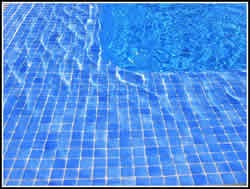
\includegraphics[width=175bp]{superficie33}

\end{figure}
\end{task}

\begin{task}{Quadra de basquete 3$\bm{\times}$3}

Uma das novidade na programação das Olimpíadas de Tóquio será o bastquete $3\times3$. Essa modalidade surgiu com fote influência da prática do esporte nas ruas, que tem como principais características, a disputa acirrada no placar e a participação dos jovens com jogadas de efeito. Marcelo quer mobilizar seus amigos para construir uma quadra de basquete $3\times3$, na sua comunidade. Para isso resolveu fazer um esboço da quadra e calcular a área correspondente a cada cor.

\begin{figure}[H]
\centering

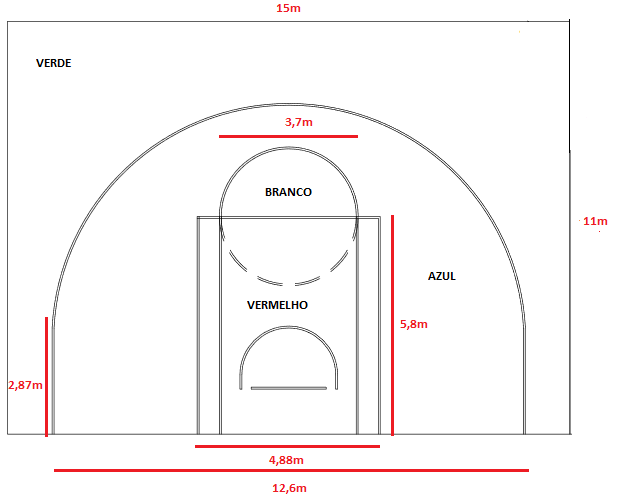
\includegraphics[width=325bp]{superficie35}

\end{figure}

Marcelo e seus amigos conseguiram arrecadar R\$$350{,}00$. Ele ainda descobriu que uma lada de $3{,}6$ litros custa $\$68{,}60$ e tem um rendimento de aproximadamente $70$m$^2$. A tinta é à base de resina acrílica para pisos cimentados, mesmo que já tenham sido pintados anteriormente. Tem grande poder de cobertura e alta durabilidade. Por isso, é muito resistente ao tráfego de pessoas, carros e intempéries, quando aplicada sobre superfícies corretamente preparadas e conservadas. Deve ser passado duas a três demãos %\url{https://loja.politintas.com.br/tinta-novacor-piso-mais-resistentesherwin-williams-3-6l/p#}
. Verifique a quantidade de tinta necessária, sabendo que vão passar duas demãos, e se é possível comprar com o valor que já foi arrecadado. Use $\pi=3{,}14$.
\end{task}

\begin{task}{a praça}
(Atividade adaptada da OBMEP - 2005)

Um prefeito quer construir uma praça quadrada de $10$m de lado, que terá canteiros triangulares iguais de pedra e um canteiro quadrado de grama, como na figura. O prefeito ainda não decidiu qual será a área do canteiro de grama, por isso o comprimento deste segmento $AB$ está indicado por $x$ na figura.

\begin{figure}[H]
\centering

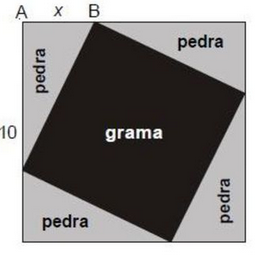
\includegraphics[width=.35\textwidth]{superficie36}
\end{figure}
\clearpage
\begin{enumerate}
  \item Calcule a área do canteiro de grama para $x=2$.
  \item Escreva a expressão da área do canteiro de grama em função de $x$.
  \item Sabe-se que o canteiro de grama custa R\$$4{,}00$ por metro quadrado, e os canteiros de pedra custam R\$$3{,}00$ por metro quadrado. Qual a menor quantia que o prefeito deve ter para construir os cinco canteiros?
\end{enumerate}
\end{task}

\clearpage
\begin{task}{Arcos de circunferência}
(UFSCar-SP) Considere a região $R$ pintada de preto exibida a seguir, construída no interior de um quadrado de lado medindo $4$cm.

\begin{figure}[H]
\centering

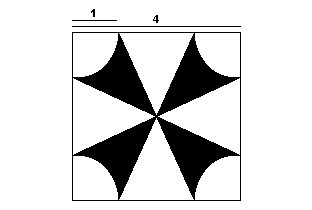
\includegraphics[width=150bp]{superficie38}
\end{figure}

Sabendo-se que os arcos de circunferência que aparecem nos cantos do quadrado têm seus centros nos vértices do quadrado e que cada raio mede $1$cm, determine a área da região $R$.
\end{task}


\begin{paginatexto}{Composição; Decomposição; Planificação}
{
\subsection{Objetivos gerais}
\begin{itemize}
\item Entender o processo de cálculo de áreas por decomposição de figuras, ou seja, saber que a área da união de partes não sobrepostas de uma figura é igual à soma de suas áreas (usar essa ideia no cálculo da diferença entre a área de uma figura e a área de uma parte contida nessa figura).
\item Analisar e avaliar casos de sólidos espaciais em que o uso de estratégias para a obtenção da área de uma superfície contida no sólido como uma parte deste, deve ser feito para a modelagem e resolução de situações do cotidiano.
\end{itemize}

\textbf{Quantidade de aulas previstas para a seção}: 10 horas/aula.

\textbf{Organização da turma}: Grupos de até 4 alunos. Socialização das respostas com todos os alunos.

\subsection{Enriquecimento da discussão}: Caro professor, nesta seção é o momento para a consolidação, a ampliação e o aprofundamento das aprendizagens essenciais desenvolvidas no capítulo. Utilizar a decomposição da superfície em polígonos e/ou setores circulares, remanejar partes da figura para compor outra e determinar áreas por excesso ou por falta estão fortemente associadas ao desenvolvimento dessa habilidade. 

Conforme \citet{BNCC2019} essa habilidade deve desenvolver à interpretação, construção de modelos, resolução e formulação de problemas matemáticos envolvendo noções, conceitos e procedimentos geométricos, entre outros. É importante destacar que o uso de estratégias para a obtenção da área de uma superfície deve ser feito para a modelagem e resolução de situações em contexto, e não apenas como procedimento técnico.

\begin{quote}
No caso da resolução e formulação de problemas, é importante contemplar contextos diversos (relativos tanto à própria Matemática, incluindo os oriundos do desenvolvimento tecnológico, como às outras áreas do conhecimento). Não é demais destacar que, também no Ensino Médio, os estudantes devem desenvolver e mobilizar habilidades que servirão para resolver problemas ao longo de sua vida – por isso, as situações propostas devem ter significado real para eles. Nesse sentido, os problemas cotidianos têm papel fundamental na escola para o aprendizado e a aplicação de conceitos matemáticos, considerando que o cotidiano não se refere apenas às atividades do dia a dia dos estudantes, mas também às questões da comunidade mais ampla e do mundo do trabalho \citep[p. 535]{BNCC2019}.
\end{quote}

Também destacamos a importância de relacionar esta seção com a habilidade (\textbf{EM13MAT309}) que consiste em resolver e elaborar problemas que envolvem o cálculo de áreas totais e de volumes de prismas, pirâmides e corpos redondos em situações reais, em particular para esta seção, as áreas totais por meio da planificação dos sólidos, quando possível.
Diversificar a abordagem metodológica é bastante favorável para um melhor desempenho dos alunos, especificamente àqueles com maiores dificuldade no raciocínio lógico-matemático. A aprendizagem da Geometria por meio de planificações amplia as condições de aprendizagem, visto que a visualização corrobora uma motivação aos alunos, proporcionando assim uma maior disposição em aprender os conteúdos propostos.
}
\end{paginatexto}

\cleardoublepage
\def\currentcolor{session1}
\begin{objectives}{Comparando embalagens}
{
Entender a área de superfície de um prisma e de um cilindro como composição de figuras planas. 
}{1}{1}
\end{objectives}
\begin{sugestions}{Comparando embalagens}
{
Convide os alunos a planificarem os sólidos no papel, para que consigam visualizar a área como uma composição de figuras planas. Verifique seus conhecimentos prévios sobre cilindros, em especial, e anote suas estratégias para a obtenção da área da lata. Socialize as respostas em grande grupo. Uma boa estratégia metodológica é, a partir das planificações, solicitar aos alunos a construção dos sólidos. Explore os sólidos construídos a fim de reconhecer a área da base, a área lateral e a área total. Questione os alunos sobre o que acontece com a área total de um prisma, quando o polígono da base for regular e apresenta diferente números de lados. A partir da planificação do cilindro, desafie os alunos a encontrarem uma forma de calcular a sua área lateral e a sua área total.

\textbf{Material necessário}: Embalagem de leite condensado (lata e caixa), Calculadora, Régua, Folha de caderno.

}{1}{1}
\end{sugestions}
\begin{answer}{Comparando embalagens}
{
A embalagem que apresenta a menor quantidade de material será a embalagem que apresentar a menor área total. Calculando a área da superfície da lata, temos:
\begin{itemize}
\item Área da base: $A_b=\pi\cdot(3,{,}25)^2\cong33{,}2$cm²  
\item Área Lateral: $A_l=2\cdot\pi\cdot3{,}25\cdot9,5\cong193,9$cm²
\item Área Total: $2\cdot A_b+A_l=2\cdot33{,}2+193{,}9=260{,}3$cm²
\end{itemize}

Calculando a área da superfície da caixa, temos:
\begin{itemize}
\item Área da base: $A_b=6{,}2\cdot4=24{,}8$cm²
\item Área Lateral: $A_l=2\cdot6{,}2\cdot12+2\cdot4\cdot12=244{,}8$cm²
\item Área Total: $2\cdot A_b+A_l=2\cdot24{,}8+244{,}8=294{,}4$cm²
\end{itemize}
Portanto, a lata apresenta a menor quantidade de material.
}{0}
\end{answer}
\begin{objectives}{Almofada para leitura}
{
Entender a área de superfície de diferentes prismas como composição de figuras planas. 
}{1}{1}
\end{objectives}
\begin{sugestions}{Almofada para leitura}
{
Esta atividade exige o conhecimento prévio do Teorema de Pitágoras. Também seria interessante conversar com alunos que a maioria dos tecidos tem $1{,}5$m de largura. Oriente os alunos a desenhar a planificação do sólido, para facilitar a resolução
}{1}{1}
\end{sugestions}
\clearmargin
\begin{answer}{Almofada para leitura}
{
Calculando a área da superfície da almofada, temos:

\textbf{Para o apoio de braço}: Área Total$=0{,}13\times0{,}1\times2+ 0{,}13\times 0{,}5 \times 2 + 0{,}1 \times 0{,}5 \times 2= 0{,}256$m²

\textbf{Para a base}: Área do retângulo da base$=0{,}43 \text{m} \times 0{,}3 \text{m} = 0{,}129$m². Área do retângulo da lateral$=0{,}43 \text{m} \times 0{,}5 \text{m} = 0{,}215$ m². Área do Triângulo $= (0{,}3 m \times 0{,}5 \text{m}) / 2=0{,}075$m².

Aplicando Pitágoras, temos: $x^2 = 30^2 + 50^2$, isto é, $x=58{,}3$cm. Assim a área do retângulo será $0{,}43\times0{,}583 \text{m}=0{,}25$m².

Logo, a área total é $0{,}129 + 0{,}215 + 2 \times 0{,}075 +0{,}25 = 0{,}744$m².

Para toda a almofada precisaremos $2 \times 0{,}256 + 0{,}744 = 1{,}256$ (m²).

Dessa forma, devemos encontrar um retângulo que tenha $1{,}5$m de largura e cuja área seja $1{,}256$m², isto é $1,256= x\cdot1{,}5$, ou ainda, $x=0{,}84$m. Considerando que a costureira costuma deixar $1$cm para costurar, o mais sensato é comprar $1$m de tecido com $1{,}5$m de largura.

}{1}
\end{answer}
\begin{objectives}{A barraca de camping}
{
  Entender a área de superfície de uma pirâmide como composição de figuras planas
}{1}{2}
\end{objectives}
\begin{sugestions}{A barraca de camping}
{
Verifique seus conhecimentos prévios sobre pirâmides, e anote suas estratégias para a obtenção da área da barraca. Explore pirâmides regulares de diferentes bases, para que os alunos percebam que as faces laterais são triângulos isósceles ou equiláteros, a fim de que concluam que a área lateral será a soma das áreas dos triângulos, que são faces laterais cuja altura é o apótema da pirâmide. A partir do Teorema de Pitágoras, desafie os alunos a expressar fórmulas para determinar o apótema da base ($a$), o apótema da pirâmide ($A$), a aresta da face lateral ($a_l$) e a sua altura ($h$). Socialize as respostas em grande grupo. 

\textbf{Material necessário}: Folha de caderno ou A4, calculadora.

}{1}{2}
\end{sugestions}
\clearmargin
\begin{answer}{A barraca de camping}
{
  Observe que temos uma pirâmide de base retangular. Calculando a área da superfície da pirâmide, temos: Área da base: $A_b=2\times2{,}35=4,7$m²

Note que a lateral é formada por dois triângulos isósceles diferentes, um de base $2$m e outro de base $2{,}35$m. Note que o apótema da face lateral da pirâmide é a altura do triângulo isósceles de uma face lateral (Figura 1). Dessa forma temos o triângulo retângulo formado pela altura da pirâmide, pelo apótema da face lateral ($A_1$  e $ A_2$) e pelo apótema da base (Figura 2), temos:

\begin{figure}[H]
\centering

\resizebox{.9\linewidth}{!}
{
  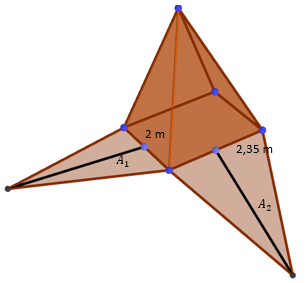
\includegraphics[height=200bp]{superficie-professor15}
  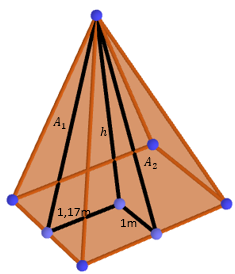
\includegraphics[height=200bp]{superficie-professor16}
}

\vspace{.3em}
Figura 1 \hspace{.3\linewidth} Figura 2
\end{figure}

$(A_1)^2=1{,}35^2+1{,}17^2$ ou ainda $A_1=1{,}79$m $(A_2)^2=1{,}35^2+1^2$ ou ainda $A_2=1{,}68$m 

Desse modo, a área lateral será a soma das áreas desses triângulos, ou ainda:
\begin{equation*}
A_l=2\times\frac{2{,}35\times1{,}79}{2}+2\times\frac{1{,}68\times2}{2}=7{,}6\text{m²}.
\end{equation*}

Calculando a área total, temos: 
\begin{equation*}
A_t=A_b+A_l=4{,}7+7{,}6=12{,}3\text{m²}.
\end{equation*}

}{1}
\end{answer}
\begin{objectives}{Quanto você tem de pele?}
{
\begin{itemize}
\item Aplicar a área da superfície de sólidos geométricos já estudados em situações do cotidiano.
\item Avaliar as relações existentes entre área de superfície e outras grandezas(comprimento), para obter aproximações para a superfície da pele de um ser humano.
\end{itemize}
}{1}{1}
\end{objectives}
\begin{sugestions}{Quanto você tem de pele?}
{\setlist[enumerate]{label=wide,left=0pt,label=\protect\bfseries\textcolor{\currentcolor}{\alph*)}}

Neste experimento faremos aproximações para descobrir quantos m² um ser humano tem de pele. Para isso, os alunos escolherão sólidos geométricos que se assemelham às partes do corpo e então, depois de calcular a área da superfície destas figuras, obterão um valor estimado para a área da pele. Discuta com a classe se é possível calcular a área da superfície da pele usando matemática e obter valores precisos. Esta discussão deve terminar com a ideia de aproximar cada parte do corpo a um sólido de área de superfície conhecida e, assim, conseguir uma estimativa da área da pele. Em seguida, peça aos alunos para imaginarem uma forma geométrica para representar a cabeça, o pescoço, as pernas, os braços, os pés e o tronco de uma pessoa. Em seguida, calcularemos a área da superfície de cada um deles obtendo, assim, uma aproximação para o tamanho da pele. Por fim, faremos uma comparação dessa medida com o valor obtido através de uma fórmula utilizada pela medicina. Pode ser interessante discutir algumas aplicações da área da pele. A principal delas é sua utilização no cálculo da dosagem de remédios, como acontece na quimioterapia, por exemplo. Mais informações sobre o experimento você consegue em \url{https://m3.ime.unicamp.br/recursos/1032}.

Acreditamos que uma das dificuldades que os alunos podem apresentar é quanto ao cone e a esfera, pois não apresentamos atividades especificas sobre o assunto. Porém, deixaremos aqui algumas sugestões de como o colega pode abordar o assunto. Para a área lateral e área total do cone sugerimos uma atividade, a partir da observação do cone desenhado e de sua planificação. Construa um cone de $6$cm de raio e $8$cm de altura. Planificando-o, verifica-se que se obtém um setor circular de raio $g$ (superfície lateral do cone) e um círculo (sua base) de raio $6$cm. Discuta com os alunos e significado de cada informação da figura e desafia-los a construírem um cone a partir de sua planificação, seguindo o roteiro:

\begin{enumerate}
\item Calcular $g$;
\item Recortar dois círculos de raio $r$ para a base do cone e outro de raio $g$ para obter o setor (a superfície lateral) do cone;
\item Calcular o ângulo $\theta$;
\item No círculo de raio g, tomando o centro como $V$ (vértice do cone), marcar o ângulo $\theta$ com o auxílio do transferidor, deixando uma sobra para colagem.
\begin{figure}[H]
\centering

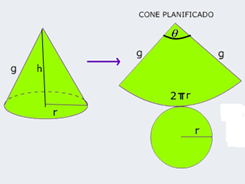
\includegraphics[width=.5\linewidth]{superficie-professor13}
\end{figure}
\end{enumerate}

 
O professor, como mediador, deverá lançar o problema e, com questionamentos, estimular os alunos a perceberem que, 

\begin{itemize}
\item  Para calcular $g$, deverão utilizar o teorema de Pitágoras;
\item Para o cálculo de $\theta$, usa-se uma regra de três;
\item Para marcar o ângulo $\theta$ e delimitar o setor circular, tem-se que, a partir de um raio $g$, considerar o centro do círculo como o vértice do cone.
\end{itemize}

\begin{multicols}{2}
\centering
Comprimento do arco
\begin{align*}
2\pi g\\
2\pi r
\end{align*}

\columnbreak
Ângulo central
\begin{align*}
3&60^{\circ}\\
&\theta
\end{align*}
\end{multicols}
No site (\url{https://m3.ime.unicamp.br/recursos/1032}) você encontra mais sugestões para tronco de cone, esfera e outros sólidos. Também gostaríamos de registrar, que no Organizando desta seção, será disponibilizado link de Geogebra, como opção para o colega que queira explorar estes conceitos com o auxílio do software.

\textbf{Material necessário}: Calculadora, fita métrica.
}{0}{9}
\end{sugestions}
\clearmargin
\begin{answer}{Quanto você tem de pele?}
{
  \begin{enumerate}
  \item Esta discussão deve terminar com a ideia de aproximar cada parte do corpo a um sólido de área de superfície conhecida e, assim, conseguir uma estimativa da área da pele. 
  \item Os itens desta tabela podem variar de acordo com a discussão com cada classe. Este é apenas um exemplo

  \begin{table}[H]
  \centering
  \begin{tabular}{|c|c|}
  \hline
  \tcolor{Partes do corpo} & \tcolor{Forma geométrica semelhante} \\
  \hline
  Cabeça & Esfera \\
  \hline
  Pescoço & Cilindro \\
  \hline
  Braços & Tronco do cone \\
  \hline
  Mãos & Cilindro \\
  \hline
  Tronco & Dois troncos de cone \\
  \hline
  Pernas & Tronco de cone \\
  \hline
  Pés & Cilindro \\
  \hline
  \end{tabular}
  \end{table}

  \item Este é apenas um exemplo. Altura: $152$cm; Peso: $51$kg.
  % \end{enumerate}

  \begin{minipage}{.6\linewidth}
  A aluna escolheu dois troncos de cone como modelo de seu tronco, a esfera como modelo da cabeça, troncos de cone para braços e pernas, e cilindros para o pescoço, pés e mãos.

  Devem ser medidos na altura do seio, cintura, distância da cintura até o quadril, circunferência da coxa, circunferência do tornozelo, circunferência do braço, do punho, comprimento do diâmetro da cabeça.
  \end{minipage}
  \begin{minipage}{.3\linewidth}
  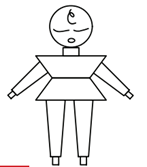
\includegraphics[width=\linewidth]{superficie-professor14}
  \end{minipage}

  % \begin{enumerate}\setcounter{enumi}{3}
  \item Neste exemplo, apresentamos as medidas que serão feitas pelos estudantes e as áreas dos sólidos.

  \begin{table}[H]
  \centering

  \begin{tabular}{|d{.3\linewidth}|d{.275\linewidth}|d{.3\linewidth}|}
  \hline
  \tcolor{Sólido Geométrico} & \tcolor{\centering Fórmula para a área de superfície} & \tcolor{Valor obtido da área} \\ 
  \hline
  Esfera & $A=\pi r^2$ & $1143$cm² \\
  \hline
  Cilindro (sem as bases) & $A=2\pi rh$ & $224$cm² \\
  \hline
  Tronco de cone & $A=\pi(R+r)g$ & $4203$cm² \\
  \hline
  Cilindro (sem as bases) & $a=2\pi r h$ & $2584$cm² (cada perna) \\
  \hline
  Tronco de cone (2) & $A=\pi(R+r)g$ & $506$cm² (em cada pé) \\
  \hline 
  Tronco de cone & $A\pi(R+r)g$ & $1003$cm² (cada braço) \\
  \hline
  Cilindro & $A=1\pi rh$ & $250$cm² (cada mão) \\
  \hline
  \tmcol{2}{|c|}{Área total da superfície da pele} & $14258$cm²\\
  \hline
  \end{tabular}
  \end{table}
  \end{enumerate}
}{1}
\end{answer}

\begin{sugestions}{Para Refletir}
{
  Uma maneira de comparar esses resultados é através da porcentagem que a diferença entre os valores representa em relação ao valor obtido pela fórmula. Socialize os dados obtidos pelos grupos para ver quem mais se aproximou.
}{0}{9}
\end{sugestions}


\explore{Composição; Decomposição; Planificação}

\begin{task}{comparando embalagens}

Uma marca de leite condensado comercializa seus produtos em duas embalagens diferentes, mas ambas com $395$g. A embalagem cilíndrica tem $6{,}5$cm de diâmetro na base e $\times$ $9{,}5$cm de altura, e a outra embalagem tem a forma de um paralelepípedo retângulo de medidas $6{,}2\text{cm}\times4{,}0\text{cm}\times12{,}0\text{cm}$.

\begin{figure}[H]
\centering

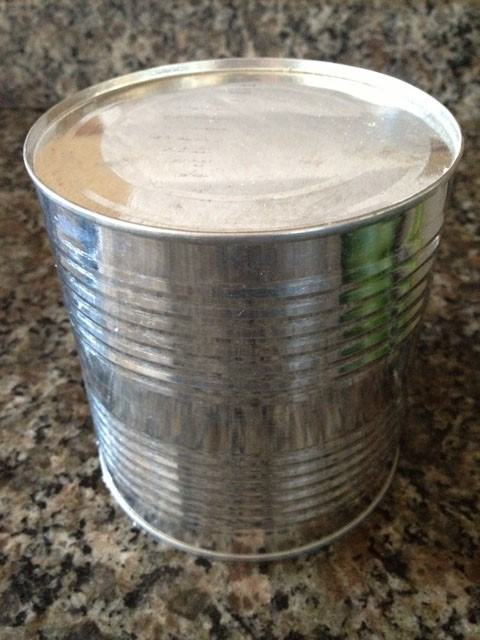
\includegraphics[height=200bp]{superficie39}\hspace{1cm}
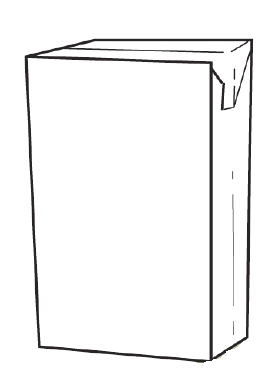
\includegraphics[height=200bp]{superficie40}

\end{figure}

Qual das embalagens apresenta a menor quantidade de material?

\end{task}
\begin{task}{almofada para leitura}
Helena gosta muito de ler na sua cama e está procurando uma almofada que lhe dê  mais conforto. Aos pesquisar na internet encontrou a seguinte descrição:

\begin{wrapfigure}[10]{l}{.35\textwidth}
\vspace{-1em}
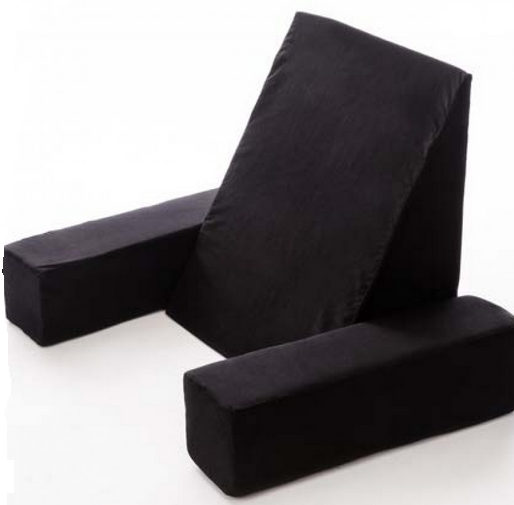
\includegraphics[width=.35\textwidth]{superficie41}
\end{wrapfigure}
\textit{"A almofada triangular é indicada para acomodar melhor o usuário na cama ou sofá, proporcionando maior conforto e diminuindo as dores nas costas. Pode ser utilizada para assistir tv e para leitura. Em pós cirúrgico para manter o tronco elevado em relação a parte inferior ou mesmo os pés mais elevado para auxiliar na circulação sanguínea e também para pessoas que necessitam passar por longos períodos em uma cama sem movimento fowler, elevação de cabeça e pés"}
\flushright
(\href{https://www.mobraz.com.br/produto/almofada-triangular-para-leitura-perfetto}{Loja Mobraz})
\justify
\clearpage
Como ela conhece uma costureira muito criativa, enviou a foto e as seguintes medidas:
\begin{itemize}
  \item Dimensões da almofada de encosto: $43\text{cm}\times50\text{cm}\times30\text{cm}$;
  \item Dimensões do apoio de braço: $13\text{cm}\times10\text{cm}\times50\text{cm}$
\end{itemize}
\noindent Calcule a quantidade mínima de tecido que Helena deve levar para a costureira.
\end{task}

\begin{task}{a barraca de camping}
O Movimento Escoteiro foi fundado em 1907, na Inglaterra, por Robert Baden-Powell, condecorado militar britânico que iniciou como uma proposta de atividades ao ar livre para grupos de jovens na Inglaterra do início do século vinte, hoje segue em constante atualização no mundo em que vivemos, com foco principal no protagonismo e no envolvimento juvenil. Através de um programa educativo baseado na Lei e na Promessa Escoteira, o escotismo foi, e ainda é, um dos maiores movimentos de educação não formal para jovens do mundo. 

O escotismo pode ser considerado como um grande jogo ao ar livre, onde os jovens dividem-se em pequenos grupos, as patrulhas ou matilhas, e realizam diversas atividades que lhes dão a oportunidade de desenvolver habilidades e conhecimentos. São acampamentos, jornadas, trilhas, aventuras e desafios em grupo que a cada dia os tornam mais empoderados e cientes das suas responsabilidades, tornando-os cidadãos ativos dentro e fora do escotismo.

\begin{figure}[H]
\centering

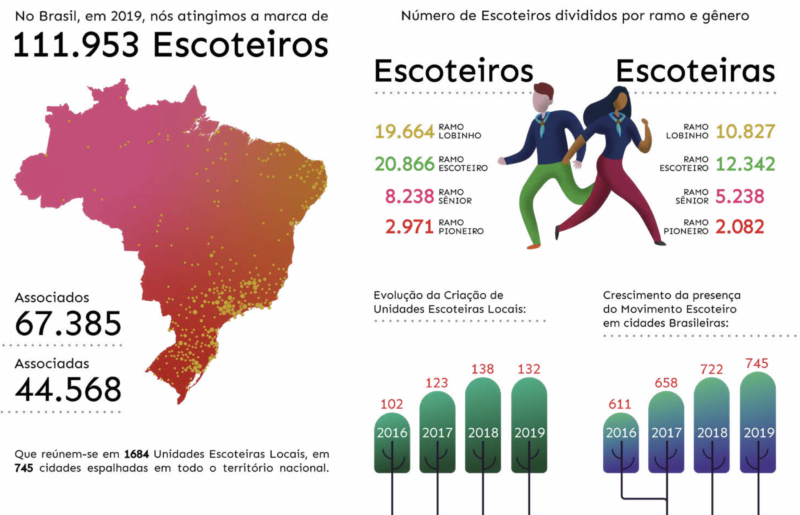
\includegraphics[width=325bp]{superficie42}

\caption{Fonte: \href{https://www.escoteiros.org.br/wp-content/uploads/2020/07/1.1.1-Foto-Gráfico-1-800x515.png}{Escoteiros do Brasil}}
\end{figure}

João e Luiza são da tropa Sênior. O Ramo Sênior é formado por jovens com idades entre 15 e 17 anos, que incentiva a superar os próprios desafios! Com a tropa sênior vivemos verdadeiras aventuras: fazemos rapel, navegamos, acampamos por vários dias, fazemos trilhas e escaladas, aprendemos jogos e atividades mais desafiadoras e somos incentivados a superar obstáculos.

Como parte do seu desafio, você ainda vai precisar de 10 noites acampado com sua patrulha ou tropa do Ramo Sênior, conquistar o cordão dourado, uma das Insígnias de Interesse Especial e uma das Insígnias da Modalidade do seu atual Ramo. Ao chegar no acampamento, a tropa foi surpreendida pelo desafio "\textit{Apresente a área total de sua barraca em m$^2$. O primeiro que acertar o resultado ganha o prêmio de 100 pontos}". Sabendo que a barraca de João e Luiza está apresentada na figura abaixo, determine a área total da barraca.
\begin{figure}[H]
\centering

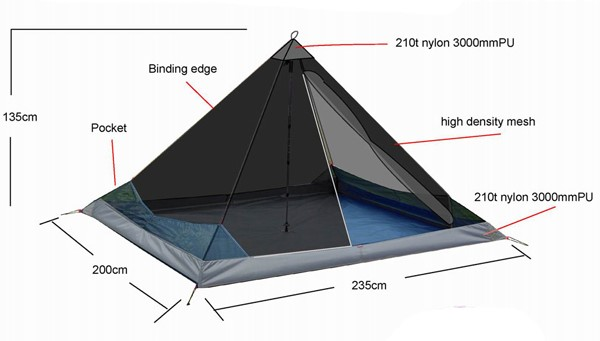
\includegraphics[width=350bp]{superficie43}
\end{figure}
\end{task}

\begin{task}{Quanto você tem de pele?}
(Atividade adaptada de \href{https://m3.ime.unicamp.br/recursos/1032}{IME-Unicamp})

\begin{wrapfigure}[10]{r}{.4\textwidth}
\vspace{-1.2em}
\includegraphics[width=.4\textwidth]{superficie44}

\caption{Fonte: \href{https://escolaeducacao.com.br/pele-humana/}{Escola Educação}}
\end{wrapfigure}

A pele é o maior órgão do corpo humano. Ela acumula várias funções como proteção, regulação da temperatura e armazenamento de energia. Além disso, a pele é responsável por grande parte das informações que recebemos do ambiente ao nosso redor, isto é, as sensações de calor, pressão e tato, sem as quais nossa vida seria muito mais complicada. 

Já imaginou as consequências de não sentir o calor do fogo? Mas qual será o tamanho deste órgão que tem tantas funções importantes? Este será o desafio do experimento: calcular a área da superfície da pele humana.


\begin{enumerate}
  \item Como podemos medir a área da pele? Discuta com seu grupo e registre.
  \item Aproxime cada parte do corpo a um sólido de área de superfície conhecida. Discuta os resultados com a turma.

  \begin{table}[H]
  \centering
  
  \begin{tabular}{|c|c|}
  \hline
  \tcolor{Partes do corpo} & \tcolor{Forma geométrica semelhante} \\
  \hline
  & \\
  \hline
  & \\
  \hline
  & \\
  \hline
  & \\
  \hline
  & \\
  \hline
  & \\
  \hline
  & \\
  \hline
  \end{tabular}
  \end{table}
  \item Escolha um membro do grupo para ser o modelo
  \begin{itemize}
    \item Decida qual sólido geométrico representará cada parte do corpo do modelo.
    \item Quais medidas são necessárias para obter a área da superfície de cada sólido?
  \end{itemize}
  \item Agora, meça o modelo do grupo e calcule a área da superfície de cada sólido escolhido por vocês.
  \begin{table}[H]
  \centering
  
  \begin{tabular}{|c|c|c|}
  \hline
  \tcolor{Sólido Geométrico} & \tcolor{Fórmula para a área de superfície} & \tcolor{Valor obtido da área} \\ 
  \hline
  & & \\
  \hline
  & & \\
  \hline
  & & \\
  \hline
  & & \\
  \hline
  & & \\
  \hline 
  & & \\
  \hline
  & & \\
  \hline
  \tmcol{2}{|c|}{Área total da superfície da pele} & \\
  \hline
  \end{tabular}
  \end{table}
\end{enumerate}

\begin{reflection}
O método de medida da área da superfície da pele, comumente usada pelos médicos, foi desenvolvido por Frederick Mosteller (1916-2006), usando a fórmula
\begin{equation*}
A=\frac{\sqrt{h\cdot m}}{60},
\end{equation*}
onde $h$ é a altura em centímetros e $m$ é a massa em quilogramas.

Calcule a área da pele de todos os componentes do grupo usando a fórmula acima. Analise os resultados obtidos com a fórmula desenvolvida por Mosteller e o valor calculado para o aluno modelo.
\end{reflection}

\end{task}

\arrange{Composição; Decomposição; Planificação}
Para calcular a área de um polígono qualquer, basta subdividi-lo em figuras tais como triângulos, quadriláteros ou outra qualquer cuja área sabemos calcular. Desta forma, a área do polígono procurado será a soma das áreas das figuras em que o decompusemos.

Assim, o cálculo de áreas de polígonos segue as seguintes regras:
\begin{enumerate}[label=\titem{\arabic*)}]
  \item Podemos associar cada polígono $P$ um número real positivo chamado área de $P$.
  \item A área de um quadrado de lado unitário é igual a $1$.
  \item Polígonos congruentes têm áreas iguais.
  \item Se um polígono $P$ está decomposto em outros polígonos, de forma que dois quaisquer possuam em comum, no máximo pontos de seus lados, então a área de $P$ é a soma das áreas desses polígonos.
\end{enumerate}

Note que as fórmulas da seção anterior foram deduzidas a partir das propriedades acima. Se sabemos que podemos encontrar a área de uma figura plana, você acha que é possível encontrar a área de uma superficie? De fato, o que é a área de uma superfície?

Área de superfície é a área da superfície da forma tridimensional. Quase todos os objetos tridimensionais com os quais você lida são compostos de faces bidimensionais(figuras planas) que são apenas quadrados, triângulos etc., e os que são curvados como esferas terão suas próprias fórmulas especiais para a área de superfície.

\subsection{Área da superfície de prismas retos}

Prismas retos são prismas obtidos tomando, para as arestas laterais, retas perpendiculares ao plano da base. Como consequência, as faces lateriais são retângulos.
\begin{figure}[H]
\centering

\includegraphics[width=250bp]{superficie45}

\caption{Versão interativa: \url{https://www.geogebra.org/m/uz5ddyzy}}
\end{figure}

Desse modo, convencionaremos:
\begin{itemize}
  \item $A_b$: área da base -- depende do polígono da base.
  \item $A_l$: área lateral -- é a soma das áreas de retângulos cujas medidas são respectivamente as de um lado do polígono da base  ($l$) e a altura do prisma ($h$), tantas quantas forem os lados do polígono da base. Expressamos por 
  \begin{equation*}
  A_l=n\times l\times h.
  \end{equation*}
  \item $A_t$: área total da superfície -- é a soma das áreas das bases e da área lateral. Expressamos por 
  \begin{equation*}
  A_t=2A_b+A_l
  \end{equation*}
\end{itemize}

Há diversos casos particulares importantes;

\begin{itemize}
  \item Quando a base é um polígono regular, obtemos um prisma regular
  \begin{figure}[H]
  \centering

  \includegraphics[width=125bp]{superficie46}\hspace{.5em}
  \includegraphics[width=200bp]{superficie47}

  \caption{Versão interativa: \url{https://www.geogebra.org/m/Fpjf6QRq}}
  \end{figure}

  \item Quando a base é um retângulo, obtemos um paralelepípedo retângulo, onde cada face é um retângulo, assim qualquer face serve como base.
  \begin{figure}[H]
  \centering

  \includegraphics[height=80bp]{superficie48}\hspace{.5em}
  \includegraphics[height=80bp]{superficie49}\hspace{.5em}
  \includegraphics[height=80bp]{superficie50}

  \caption{Versão interativa: \url{https://www.geogebra.org/m/k8kKsFUz}}
   \end{figure}

   \item Quando a base é um quadrado e as arestas possuem a mesma medida do lado da base, obtemos um hexaedro regular (ou cubo)

   \begin{figure}[H]
   \centering

   \includegraphics[width=350bp]{superficie51}


   \caption{Versão interativa: \url{https://www.geogebra.org/m/dyz3zBwn}}
   \end{figure}
\end{itemize}

\subsection{ Área da superfície de cilindros retos}

O cilindro é chamado reto no caso em que suas geratrizes são perpendiculares aos planos das bases. O cilindro equilátero é o cilindro circular reto em que a altura é igual ao diâmetro da base.

\begin{figure}[H]
\centering

\includegraphics[height=100bp]{superficie52}\hspace{.5em}
\includegraphics[height=100bp]{superficie53}\hspace{.5em}
\includegraphics[height=100bp]{superficie54}

\caption{Versão interativa: \url{https://www.geogebra.org/m/XzfFNDYV}}
\end{figure}

Desse modo, convencionaremos:
\begin{itemize}
  \item $A_b$: área da base -- área do círculo. Expressamos por
  \begin{equation*}
  A_b=\pi r^2,
  \end{equation*}
  onde $r$ é o raio do cilindro

  \item $A_l$: área lateral -- a superfície lateral de um cilindro reto de raio $r$ e altura $h$, pode ser desenrolada e transformada em um retângulo de base $2\pi r$ e altura $h$. A área lateral do cilindro é igual à área desse retângulo, e expressamos por  
  \begin{equation*}
  A_l=2\pi rh.
  \end{equation*}
  \item $A_t$: área total da superfície -- é a soma das áreas das bases e da área lateral. Expressamos por 
  \begin{equation*}
  A_t=2A_b+A_l=2\pi r^2+2\pi rh=2\pi r(r+h)
  \end{equation*}
\end{itemize}

O cilindro circular reto é também chamado de cilindro de revolução, por ser gerado pela rotação completa de um retângulo por um de seus lados. Assim, a rotação do retângulo pelo lado gera o cilindro mostrado.

\begin{figure}[H]
\centering

\includegraphics[height=150bp]{superficie55}\hspace{.5em}
\includegraphics[height=150bp]{superficie56}\hspace{.5em}
\includegraphics[height=150bp]{superficie57}

\caption{Versão interativa: \url{https://www.geogebra.org/m/nh2xNMe7}}
\end{figure}

\subsection{ Área da superfície de pirâmides retas}

Uma pirâmide reta é aquela cuja projeção ortogonal do vértice sobre o plano da base é o centro da base.

\begin{figure}[H]
\centering

\includegraphics[height=150bp]{superficie58}\hspace{.5em}
\includegraphics[height=150bp]{superficie59}

\caption{Versão interativa: \url{https://www.geogebra.org/m/cdxwhx4t}}
\end{figure}

Desse modo, convencionaremos:
\begin{itemize}
  \item $A_b$: área da base -- depende da figura que temos como polígono da base.
  \item $A_l$: área lateral -- a superfície lateral de uma pirâmide é formada por $n$ triângulos cuja base tem a mesma medida do lado do polígono da base, e a altura é o apótema (A) da face lateral da pirâmide. A área lateral da pirâmide é igual à $n$ vezes a área desse triângulo, e expressamos por
  \begin{equation*}
  A_l=\frac{nAl}{2}.
  \end{equation*}
  \item $A_t$: área total da superfície -- é a soma das áreas das bases e da área lateral. Expressamos por 
  \begin{equation*}
  A_t=A_b+A_l
  \end{equation*}
\end{itemize}

Pirâmide regular é uma pirâmide cuja base é um posígosno regular e a projeção ortogonal do vértice sobre o plano da base é o centro da pirâmide. Uma pirâmide regular possui arestas laterais congruentes e as faces laterais são triângulos isósceles.

\begin{figure}[H]
\centering

\includegraphics[height=140bp]{superficie60}\hspace{.5em}
\includegraphics[height=140bp]{superficie61}
\end{figure}

Dessa forma, valem as seguintes relações para as pirâmides regulares retas, quando a apótema do triângulo isósceles que seja uma face lateral é também chamado de geratriz da pirâmide:
\begin{itemize}
  \item $(a_l)^2=A^2+\bigg(\dfrac{l}{2}\bigg)^2$, onde $a_l$ representa a aresta lateral, $A$ é a geratriz ou apótema e $l$, é o lado da base.
  \item $A^2=h^2+a^2$, onde $a$ representa o apótema da base, $A$ é a geratriz ou apótema, e $h$ é a altura da pirâmide.
\end{itemize}

\begin{figure}[H]
\centering

\includegraphics[height=140bp]{superficie62}
\end{figure}

\subsection{ Área da superfície de cones retos}

Em um cone, a base não precisa ser um polígono, mas qualquer região plana delimitada por uma curva fechada. Os cones mais importantes são os cones circulares, em que a base é um círculo. Um cone é equilátero quando a medida da geratriz é igual à medida do diâmetro da base.

\begin{figure}[H]
\centering

% \resizebox{\textwidth}{!}
{\includegraphics[height=100bp]{superficie63}\hspace{.5em}
\includegraphics[height=100bp]{superficie64}\hspace{.5em}
\includegraphics[height=100bp]{superficie65}}

\caption{Versão interativa: \url{https://www.geogebra.org/m/yzGzrUxs}}
\end{figure}

Desse modo, convencionados

\begin{itemize}
  \item $A_b$: área da base -- área do círculo de raio $r$. Expressamos por
  \begin{equation*}
  A_b=\pi r^2
  \end{equation*}  
  \item $A_l$: área lateral -- a superfície lateral de um cone de raio $r$ e geratriz $g$, pode ser desenrolada e transformada em um setor de raio $g$, cujo arco tem comprimento $2\pi r$. A área deste setor é igual à área lateral do cone, e para calculá-la usaremos proporcionalidade. Diremos que
  \begin{equation*}
  \frac{\text{área do setor}}{\text{área do círculo}}=\frac{\text{comprimento do arco}}{\text{comprimento da circunferência}},
  \end{equation*}
  ou ainda,
  \begin{equation*}
  \frac{A_l}{\pi g^2}=\frac{2\pi r}{2\pi g}.
  \end{equation*}
  Expressamos por $A_l=\pi rg$.
  \item $A_t$: área total da superfície -- é a soma da área da base e da área lateral. Expressamos por
  \begin{equation*}
  A_t=A_b+A_l=\pi r^2+\pi rg=\pi r(r+g).  
  \end{equation*}
\end{itemize}

Um cone circular reto também é chamado de cone de revolução, por ser gerado pela rotação de um triângulo retângulo em torno do eixo dado por um dos catetos.

\begin{figure}[H]
\centering

\includegraphics[height=125bp]{superficie66}\hspace{.5em}
\includegraphics[height=125bp]{superficie67}\hspace{.5em}
\includegraphics[height=125bp]{superficie68}

\caption{Versão interativa: \url{https://www.geogebra.org/m/deyt2w4u}}
\end{figure}

Para o cone reto, todos os segmentos que formam sua superfície lateral têm a mesma medida. Esse segmento comum é a geratriz do cone, denotada por $g$ e sua medida, e sua medida satisfaz a relação 
\begin{equation*}
g^=h^2+r^2
\end{equation*}

Vamos considerar o tronco de cone reto como sendo a parte do cone compreendida entre o plano que contém a base do cone e outro plano paralelo a esse, que secciona o cone. A base do tronco é o círculo de raio $R$ e o topo é um círculo de raio $r$. Sua altura é o segmento perpendicular à base entre os dois planos. A geratriz $g$ do tronco é o segmento da geratriz $G$ do cone, compreendido entre o topo e a base.
\begin{figure}[H]
\centering

\includegraphics[width=250bp]{superficie69}

\caption{Versão interativa: \url{https://m3.ime.unicamp.br/recursos/1032}}
\end{figure}

Então, a área $A_t$ da superfície de um tronco de cone pode ser calculada como a diferença entre a área da superfície do cone inicial e a área da superfície do cone que restou após ser retirado o tronco. Veja na figura abaixo:

\begin{figure}[H]
\centering

\includegraphics[width=400bp]{superficie71}

\caption{Fonte: \href{https://m3.ime.unicamp.br/recursos/1032}{IME-Unicamp}}
\end{figure}
% \begin{figure}[H]
% \centering

% \begin{tikzpicture}
% \coordinate (A) at (0,0);
% \coordinate (V) at (0,4);
% \coordinate (B) at (2,0);
% \coordinate (G) at (1.5,3);

% \draw (A) -- (V) -- (B) -- cycle;
% \draw (G) -- +($(B)!(G)!(V)$);

% \node [fill=white] at (1.5,3) {$G$};
% \end{tikzpicture}
% \end{figure}

Assim,
\begin{equation*}
A_t=\pi(R+r)g
\end{equation*}

\subsection{ Área da superfície da esfera}

A área da superfície da esfera de raio $R$ é igual a 

\begin{equation*}
4\pi R^2.
\end{equation*}

Uma ideia para se chegar a essa fórmula é considerar a superfície da esfera como o resultado da rotação de uma semicircuferência em dorno de seu eixo.

Imaginemos a esfera dividida em infinitas \textit{cunhas} e cada uma dessas cunhas dividida em infinitas pirâmides de altura $h$ igual ao raio $r$ da esfera.

Sejam ainda $A_1,A_2,A_3,...,A_n$ as áreas das bases de cada uma dessas pirâmides.

Lembrando que

\begin{align*}
V_{\text{esf}}&=\frac{4}{3}\pi r^3\\
V_{\text{pir}}=&\frac{1}{3}A_bh.
\end{align*}

Como o volume total das pirâmide é aproximadamente o volume da esfera,

\begin{align*}
&\frac{1}{3}A_1 r+\frac{1}{3}A_2 r+\frac{1}{3}A_3r+\cdots\frac{1}{3}A_n r \approx\frac{4}{3}\pi r^3\\
&\frac{1}{3}r(A_1,+A_2+A_3+\cdots+A_n)\approx\frac{4}{3}\pi r^3.
\end{align*}

Quando $n$ tende a infinito,

\begin{align*}
\frac{1}{3}rS_3\approx\frac{4}{3}\pi r^3\\
\therefore S_3\approx4\pi r^2
\end{align*}
\begin{figure}[H]
\centering

\includegraphics[width=350bp]{superficie73}

\caption{Versão interativa: \url{https://www.geogebra.org/m/nrcwwbg3}}
\end{figure}


\clearpage
\def\currentcolor{session2}

\begin{objectives}{Planetário}
{
  Analisar e avaliar casos de sólidos espaciais em que o uso de estratégias para a obtenção da área de uma superfície deve ser feito para a modelagem e resolução de situações em contexto.
}{1}{1}
\end{objectives}
\begin{sugestions}{Planetário}
{
  A atividade tem caráter de aplicação dos conceitos construídos no Explorando, em particular o cálculo da área da superfície esférica. Para este exercício você deve reforçar a diferença entre semiesfera e semicírculo.
}{1}{1}
\end{sugestions}

\begin{objectives}{Telhado}
{
  Analisar e avaliar casos de sólidos espaciais em que o uso de estratégias para a obtenção da área de uma superfície deve ser feito para a modelagem e resolução de situações em contexto.
}{1}{1}
\end{objectives}
\begin{sugestions}{Telhado}
{
  A atividade tem caráter de aplicação dos conceitos construídos no Explorando, em particular o cálculo da área da superfície de prismas. Para este exercício você desconsiderar a estrutura do telhado.
}{1}{1}
\end{sugestions}


\begin{answer}{Planetário}
{
  Calculando a área da superfície da semiesfera, temos:
\begin{equation*}
  A_1=\frac{4\times\pi\times14^2}{2}=1176\text{m²}.
\end{equation*}
Calculando a área do semicírculo, temos: 
\begin{equation*}
A_2=\frac{\pi\times3^2}{2}=13{,}5\text{m²}.
\end{equation*}
Assim, a área da cobertura será
\begin{equation*}
A_1-12A_2=1176-12\times13{,}5=1014\text{m²}.
\end{equation*}
Sabendo que 1 lata de tinta é suficiente para $39$m², então precisamos de, no mínimo, 26 latas de tinta.

\tcbsubtitle{Telhado}

Para responder essa questão, precisamos encontrar a medida "$a$" do telhado. Utilizando o teorema de Pitágoras, no triângulo da extremidade, temos: $a^2= 4^2+ 3^2$ e, assim $a = 5$m.

Agora temos as duas medidas que formam cada uma das partes do telhado. O telhado é composto por dois retângulos, cujas dimensões são 5 metros e 30 metros.

Assim, área telhado $= 2 x 30 x 5 = 300$m²

A dimensões de cada telha são: $0{,}15$m por $0{,}2$m, área da telha = $0{,}15\text{m}\times0{,}2 \text{m} = 0{,}03$m²

A área do telhado, dividida pela área unitária da telha, resulta na quantidade de telhas necessárias: $n =  300/0{,}03= 10000$ telhas.

}{0}
\end{answer}

\clearmargin

\begin{objectives}{Comprimidos de remédios}
{
  Analisar e avaliar casos de sólidos espaciais em que o uso de estratégias para a obtenção da área de uma superfície deve ser feito para a modelagem e resolução de situações em contexto.
}{1}{2}
\end{objectives}
\begin{sugestions}{Comprimidos de remédios}
{
  A atividade tem caráter de aplicação dos conceitos construídos no Explorando, em particular o cálculo da área da superfície de cilindros.
}{1}{2}
\end{sugestions}
\begin{answer}{Comprimidos de remédios}
{
  Para o primeiro comprimido devemos considerar o cilindro e uma esfera (duas semiesferas em cada ponta) de raio 0,25 cm. Assim, temos:

\begin{itemize}
\item Área do cilindro:  $A_c=2\times\pi\times0{,}25\times1{,}5=2{,}35$cm²
\item Área da esfera: $A_e=4\times\pi\times0{,}25^2=0{,}785$cm².
\end{itemize}
Logo, a área da superfície do primeiro comprimido é $2,35+0,785=3,135$cm²

No segundo comprimido temos um cilindro de altura 0,5 cm e cuja área deve ser 3,135 cm².

Assim,      
\begin{align*}
2\times\pi\times r^2+2\times\pi\times r\times0{,}5=&3{,}135\\
6{,}28 r^2+3{,}14 r-3{,}135=&0
\end{align*}
Resolvendo a equação encontramos $r_1=0{,}5$. Observe que só consideramos a raiz positiva.
Assim, o diâmetro deve ser de $1$cm.
}{1}
\end{answer}

\practice{Composição; Decomposição; Planificação}
\begin{task}{Planetário}

(UFSM - 2011) Oscar Niemayer é um arquiteto brasileiro, considerado um dos nomes mais influentes na arquitetura moderna internacional. Ele contribuiu, através de uma doação de um croqui, para a construição do planetário da UFSM, um marco arquitetônico importante da cidade de Santa Maria.

\begin{figure}[H]
\centering

\includegraphics[width=275bp]{superficie76}

\end{figure}

Suponha que a cobertura da construção seja uma semiesfera de $28$m de diâmetro, vazada por 12 parte iguais, as quais são aproximadas por semicírculos de raio $3$m. Sabendo que uma lata de tinta é suficiente para pintar $39\text{m}^2$ de área, qual a quantidade mínima de latas de tinta necessária para pintar toda a cobertura do planetário? (use $\pi=3$).

\end{task}

\begin{task}{telhado}
\begin{wrapfigure}{r}{.5\textwidth}
\centering
\includegraphics[width=.5\textwidth]{superficie77}

\end{wrapfigure}
(PUC RS/2012) A quantidade de materiais para executar uma obra é essecial para prever o custo da construção. Quer-se construir um telhado cujas dimensões e formato são indicados na figura abaixo.

A quantidade de telhas de tamanho $15$cm por $20$cm necessárias para fazer esse telhado é:


\end{task}

\clearpage

\begin{task}{comprimidos de remédios}

(Faap) A razão na qual um comprimido de vitamina C começa a dissolver-se depende da área da superfície do comprimido. Uma marca de comprimido tem forma cilíndrica, comprimento $2$ centímetros, com hemisférios de diâmetro $0{,}5$ centímetro cada extremidade, conforme a figura a seguir. Uma segunda marca de comprimido avai ser fabricada em forma cilíndrica, com $0{,}5$ centímetro de altura.

\begin{wrapfigure}{r}{.4\textwidth}
\centering

\includegraphics[width=.4\textwidth]{superficie78}
\end{wrapfigure}
Determine o diâmetro do segundo comprimido de modo que a área da superfície seja igual à do primeiro comprimido.

\begin{enumerate}
  \item $2{,}0\text{cm}$
  \item $1{,}5\text{cm}$
  \item $2{,}5\text{cm}$
  \item $0{,}5\text{cm}$
  \item $1{,}0\text{cm}$
\end{enumerate}
\end{task}

\exercise

\begin{answer}{Exercícios}
{\exerciselist
  \begin{enumerate}
  \item Letra A
  \end{enumerate}
}{1}
\end{answer}
\clearmargin
\begin{answer}{Exercícios}
{\exerciselist
  \begin{enumerate}\setcounter{enumi}{1}
  \item Letra A
  \item Letra B
  \item Letra C
  \end{enumerate}
}{1}
\end{answer}
\clearmargin
\begin{answer}{Exercícios}
{\exerciselist
  \begin{enumerate}\setcounter{enumi}{4}
  \item Letra D
  \item Letra B
  \end{enumerate}
}{1}
\end{answer}
\clearmargin
\begin{answer}{Exercícios}
{\exerciselist
  \begin{enumerate}\setcounter{enumi}{6}
  \item Letra D
  \item Letra B
  \item Letra E
  \item Letra E
  \end{enumerate}
}{1}
\end{answer}
\clearmargin
\begin{answer}{Exercícios}
{\exerciselist
  \begin{enumerate}\setcounter{enumi}{10}
  \item Letra C
  \item Letra D
  \end{enumerate}
}{1}
\end{answer}
\clearmargin
\begin{answer}{Exercícios}
{\exerciselist
  \begin{enumerate}\setcounter{enumi}{12}
  \item Letra B
  \item $S_2>S_1$
  \end{enumerate}
}{1}
\end{answer}
\clearmargin
\begin{answer}{Exercícios}
{\exerciselist
  \begin{enumerate}\setcounter{enumi}{14}
  \item Letra B
  \item $18$m²
  \item Letra E
  \end{enumerate}
}{1}
\end{answer}
\clearmargin
\begin{answer}{Exercícios}
{\exerciselist
  \begin{enumerate}\setcounter{enumi}{17}
  \item Letra E
  \item Letra B
  \end{enumerate}
}{1}
\end{answer}
\clearmargin
\begin{answer}{Exercícios}
{\exerciselist
  \begin{enumerate}\setcounter{enumi}{19}
  \item Letra D
  \item Letra C
  \item Letra C
  \end{enumerate}
}{1}
\end{answer}
\clearmargin
\begin{answer}{Exercícios}
{\exerciselist
  \begin{enumerate}\setcounter{enumi}{22}
  \item $\dfrac{2\sqrt{3}}{3}$
  \end{enumerate}
}{1}
\end{answer}

\begin{enumerate}
  \item (Fuvest/98) Considere o triângulo representado na malha pontilhada com quadrados de lados iguais a $1$cm. A área do triângulo, em cm$^2$, é
  \begin{figure}[H]
  \centering

\includegraphics[width=100bp]{superficie79}
  \end{figure}
  \begin{enumerate}
    \item 2
    \item 3
    \item 4
    \item 5
    \item 6
  \end{enumerate}

\clearpage
  \item (Canguru - 2019) No interior de cinco retângulos, geometricamente iguais, foram sombreadas regiões triangulares ou retangulares, conforme se mostra nas figuras seguintes. Em qual das figuras a parte sombreada tem a maior área?
  \begin{enumerate}
    \begin{multicols}{5}
    \item \adjustbox{valign=t}{\includegraphics[width=50bp]{superficie80}}
    \item \adjustbox{valign=t}{\includegraphics[width=50bp]{superficie81}}
    \item \adjustbox{valign=t}{\includegraphics[width=50bp]{superficie82}}
    \item \adjustbox{valign=t}{\includegraphics[width=50bp]{superficie83}}
    \item \adjustbox{valign=t}{\includegraphics[width=50bp]{superficie84}}
    \end{multicols}
  \end{enumerate}
  

  \item O retângulo $ABCD$ representa um terreno retangular cuja largura é 3/5 do comprimento. A parte hachurada representa um jardim retangular cuja largura é também 3/5 do comprimento. Qual a razão entre a área do jardim e a área total do terreno?
  \begin{figure}[H]
  \centering

  \includegraphics[width=100bp]{superficie85}
  \end{figure}
  \begin{enumerate}
    \item 30\%
    \item 36\%
    \item 40\%
    \item 45\%
    \item 50\%
  \end{enumerate}

  \item (Cefet/MG - 2016) A área quadrada de um sítio deve ser dividida em quatro partes iguais, também quadradas, e em uma delas, deverá ser mantida uma reserva de mata nativa (área hachurada, conforme mostra a figura a seguir. 
  \begin{figure}[H]
  \centering
  \includegraphics[width=150bp]{superficie86}

  \end{figure} 

  Sabendo que $B$ é o ponto médio do segmento $AE$ e $C$ é o ponto médio do segmento $EF$, a área hachurada, em m$^2$, mede
  \begin{enumerate}
    \item $625{,}0$
    \item $925{,}5$
    \item $1562{,}5$
    \item $2500{,}0$
  \end{enumerate}

\clearpage

  \item (Fuvest/99) Dois irmãos herdaram um terreno com a seguinte forma e medidas:

  \begin{multicols}{2}
  \begin{itemize}[label=]
    \item $AD=20\text{m}$;
    \item $AB=60\text{m}$;
    \item $BC=16\text{m}$;
  \end{itemize}

  \begin{figure}[H]
  \centering

  \includegraphics[width=150bp]{superficie87}
  \end{figure}
 
  \end{multicols}
   Para dividir o terreno em duas partes de mesma área, eles usaram uma reta perpendicular a $AB$. Para que a divisão seja feita corretamente, a distância dessa reta ao ponto $A$, em metros, deversá ser:
  \begin{enumerate}
    \item 31
    \item 32
    \item 33
    \item 34
    \item 35
  \end{enumerate}

  \item (ENEM - 2010) A loja Telas \& Molduras cobra 20 reais por metro quadrado de tela, 15 reais por metro linear de moldura, mais uma taxa fixa de entrega de 10 reais. Uma artista plástica precisa encomendar telas e molduras a essa loja, suficientes para 8 quadros retangulares ($25\text{cm}\times50\text{cm}$). O valor da segunda encomenda será
  \begin{enumerate}
    \item o dobro do valo da primeira encomenda, porque a altura e a largura dos quadros dobraram.
    \item maior do que o valor da primeira encomenda, mas não o dobro.
    \item a metade do valor da primeira encomenda, porque a altura e a largura dos quadros dobraram.
    \item menor do que o valor da primeira encomenda, mas não a metade.
    \item igual ao valor da primeira encomenda, porque o custo de entrega será o mesmo.
  \end{enumerate}


  \item (ENEM - 2009) Membros de uma família estão decidindo como irão dispor dduas camas em um dos quartos da casa. As camas têm $0{,}80$m de largura por $2$m de comprimento cada. As figuras a seguir expõem os esbo'xos das ideias sugeridas por José, Rodrigo e Juliana, respectivamente. Em todos os eboços, as camas ficam afastadas $0{,}20$m das paredes e permitem que a porta seja aberta em pelo menos $90^{\circ}$. José, Rodrigo e Juliana concordaram que a parte listrada em cada caso será de difícil circulação, e a área branca é de livre circulação. Entre essas propostas, a(s) que deixa(m) maior área livre para circulação é(são)
  \begin{figure}[H]
  \centering

  \includegraphics[width=300bp]{superficie88}
  \end{figure}
  \begin{enumerate}
    \item a proposta de Rodrigo.
    \item a proposta de Juliana.
    \item as propostas de Rodrigo e Juliana.
    \item as propostas de José e Rodrigo.
    \item as propostas de José, Rodrigo e Juliana.
  \end{enumerate}

  \item (ENEM - 2019) Uma pessoa de estatura mediana pretende fazer um alambrado em torno do campo de futebol de seu bairro. No dia da medida do terreno, esqueceu de levar a trena para realizar a medição. Para resolver o problema, a pessoa cortou uma vara de comprimento igual a sua altura. O formado do campo é retangular e foi constatado que ele mede 53 varas de comprimento e 30 varas de largura.

  Uma região $R$ tem área $A_R$, dada em m$^2$, de mesma medida do campo de futebol, descrito anteriormente. A expressão algébrica que determina a medida da vara em metros é
  \begin{enumerate}
    \begin{multicols}{2}
    \item Vara = $\displaystyle\sqrt{\frac{A_R}{1500}}$m
    \item Vara = $\displaystyle\sqrt{\frac{A_R}{1590}}$m
    \item Vara = $\displaystyle\frac{1590}{a_R}$m
    \item Vara = $\displaystyle\frac{A_R}{1500}$m
    \item Vara = $\displaystyle\frac{A_R}{1590}$m
    \end{multicols}
  \end{enumerate}

  \item (ENEM - 2014) O governo, num programa de moradia, num programa de moradia, tem por objetivo contruir 1 muilhão de habitações, em parceria com estados, municípios e iniciativa privada. Um dos modelos de cada popular proposto por construtoras deve apresentar $45$m$^2$ e deve ser colocado piso de cerãomica em toda sua a'rea interna. Supondo que serão construídas 100 mil casas desse tipo, deprezando-se as larguras das paredes e portas, o número de peças de cerâmica de dimensões $20\text{cm}\times20\text{cm}$ utilizadas será
  \begin{enumerate}
    \item 11,25 mil
    \item 180 mil.
    \item 225 mil.
    \item 22.500 mil.
    \item 112.500 mil.
  \end{enumerate}

  \item (ENEM - 2011) A figura que segue é formada por cinco quadrados congruentes, cuja medida do lado é $L$, e um quadrado $ABCD$ com vértices em um único vértice de quatro dos cinco quadrados. A área do quadrado $ABCD$ é equivalente à área de um retângulo de lados

  \begin{multicols}{2}
  \begin{figure}[H]
    \centering
  
    \includegraphics[width=125bp]{superficie89}
    \end{figure}
  
    \begin{enumerate}
      \item $2\ell$ e $3\ell$
      \item $3\ell$ e $1\ell$
      \item $3\ell$ e $3\ell$
      \item $4\ell$ e $1\ell$
      \item $5\ell$ e $1\ell$
    \end{enumerate}
  \end{multicols}

  \item (ENEM-2011) Em uma cidade, a cada inauguração de prédios, a orientação da prefeitura, por meio de uma lei de incentivo à cultura, é a construção de uma obra de arte na entrada ou no \textit{hall} desse prédio. Em contrapartida, a prefeitura oferece abatimento em impostos. No edifício das Acácias, o artista contratado resolveu fazer um quadrado composto de 12 mosaicos, de dimentões $12\text{cm}$ por $6$cm cada um, conforme a figura

  \begin{figure}[H]
  \centering

  \includegraphics[width=225bp]{superficie90}
  \end{figure}

  A área da figura sobreada no quadrado é de?
  \begin{enumerate}
    \item $36$cm$^2$
    \item $72$cm$^2$
    \item $144$cm$^2$
    \item $288$cm$^2$
    \item $432$cm$^2$
  \end{enumerate}

  \item (Upe-ssa 2017) Rafael decidiu colocar colocar cerâmicas com a forma de hexágonos regulares no piso da sala de seu escritório. Sabendo que a área do piso do escritório mede $25{,}5$m$^2$, que a cerâmica mede $10$cm de lado, desconsiderando a área ocupada pelos rejuntes, quantas pedras de cerâmicas serão necessárias para cobrir todo o piso dessa sala?
  \begin{figure}[H]
  \centering

  \includegraphics[width=175bp]{superficie91}
  \end{figure}

  Considere $\sqrt{3}=1{,}7$

  \begin{enumerate}
    \item 225
    \item 425
    \item 765
    \item 1000
    \item 1250
  \end{enumerate}

  \item (ENEM - 2015) O propietário de um parque aquático deseja construir uma piscina em suas dependências. A figura representa a a vista superior dessa piscina, que é formada por três setores circulares idênticos, com ângulo central igual a $60^{\circ}$. O raio $R$ deve ser um número natural.

  \begin{figure}[H]
  \centering

  \includegraphics[width=175bp]{superficie92}
  \end{figure}

  O parque aquático já conta com uma piscina em formato retangular com dimensões $50$m$\times24$m. O propietário quer que a área ocupada pela nova piscina seja menor que a ocupada pela piscina já existente. Considere $3{,}0$ como aproximação para $\pi$. O maior valor possível para $R$, em metros, deverá ser

  \begin{enumerate}
    \item 16.
    \item 28.
    \item 29.
    \item 31.
    \item 49.
  \end{enumerate}

  \item (Adaptado de Temas e Problemas) Na figura abaixo, os lados $AB$ e $AC$ do triângulo $ABC$ estão divididos em três partes iguais, onde $\displaystyle AD=\frac{2}{3}\text{ e }A=\frac{2}{3}AC$. O segmento $DE$ divide o triângulo em duas partes: um triângulo de área $S_1$ e um trapézio de área $S_2$. Qual destas duas áreas é maior?

  \begin{figure}[H]
  \centering

  \includegraphics[width=150bp]{superficie93}
  \end{figure}
\clearpage
  \item (G1 - ifpe 2017) Os alunos do curso de Xootecnia do \textit{Campus} Vitória adotaram um cachorro que sempre passeava próximo ao \textit{Campus}. A figura abaixo representa a vista frontal da casa que estão construindo para o cachorro Tobby.

  Sabendo que a casa vai ser toda construída de madeira, qual é a superfície de madeira na parede frontal da casa, de acordo com a figura a seguir (Use $\pi=3{,}14$).
  \begin{multicols}{2}
   \begin{enumerate}
    \item $4471\text{cm}^2$
    \item $5372\text{cm}^2$
    \item $6000\text{cm}^2$
    \item $7600\text{cm}^2$
    \item $6972\text{cm}^2$
  \end{enumerate}
  \begin{figure}[H]
  \centering

  \includegraphics[width=175bp]{superficie94}
  \end{figure}
  \end{multicols}

  \item (XXIX OBM) Uma sala quadrada com $81\text{m}^2$ de área tem os seu piso inteiramente coberto por dois tapetes retangulares $A$ e $B$, que não se superpõem, conforme mostrado na figura (2). Em certo momento, o tapete $B$ é deslocado, o tapete $A$ é dirado $90^{\circ}$ e colocado sobre o tapete $B$, conforme indicado na figure (2).

  \begin{figure}[H]
  \centering

  \includegraphics[width=200bp]{superficie95}
  \end{figure}

  Sabendo que a área do tapete $B$ é o dobro da área do tapete $A$, calcule a área da parte do piso que ficou descoberta.

  \item (Cesgranrio) Uma folha de papel colorido, com a forma de um quadrado de $20$cm de lado, será usada para cobrir todas as faces e a bse de uma pirâmide quadrangular regular com altura de $12$cm e apótema da base medindo $5$cm. Após se ter concluído essa tarefa, e levando-se em conta que não houve desperdício de papel, a fração percentual que sobrará dessa folha de papel corresponde a:
  \begin{enumerate}
    \item $20\%$
    \item $16\%$
    \item $15\%$
    \item $12\%$
    \item $10\%$
  \end{enumerate}
\clearpage
  \item (ENEM - 2019) Uma empresa de transporte disponibiliza, para embalagem de encomendas, caixas de papelão no formato de paralelepípeddo reto retângulo, conforme dimensões no quadro.

  \begin{table}[H]
  \centering

  \begin{tabular}{|c|c|c|c|}
  \hline
  \tcolor{Modelo da caixa} & \tcolor{Comprimento (c)} & \tcolor{Largura (cm)} & \tcolor{Altura (cm)}\\
  \hline
  1 & 12 & 12 & 13\\
  \hline
  2 & 23 & 20 & 25\\
  \hline
  3 & 25 & 25 & 25\\
  \hline
  4 & 26 & 25 & 24\\
  \hline 
  5 & 23 & 26 & 26\\
  \hline
  \end{tabular}
  \end{table}

  Para embalar uma encomenda, contendo um objeto esférico de $11$cm de raio, essa empresa adota como critério a utilização da caixa, dentre od modelos disponíveis, que comporte, quando fechada e sem deformá-la, a encomenda e que possua a menor área de superfície total.

  Desconsidere a espessura da caixa. Nessas condições, qual dos modelos apresentados deverá ser o escolhido pela empresa?
\begin{multicols}{5}
  \begin{enumerate}
    \item 1
    \item 2 
    \item 3 
    \item 4 
    \item 5
  \end{enumerate}
\end{multicols}

  \item (UERJ) Para revestir externamente chapéus em forma de cones com $12$cm de altura e diâmetro da base medindo $10$cm, serão utilizados cortes retangulares de tecido, cujas dimensões são $67$cm por $50$cm. Admita que todo o tecido de cada corte poderá ser aproveitado. O número mínimo dos referidos cortes necessários para forrar 50 chapéus é igual a
  \begin{enumerate}
    \item 3
    \item 4
    \item 5
    \item 6
  \end{enumerate}

  \item (ENEM - 2014) Uma empresa que organiza eventos de formatura confecciona canudos de diplomas a partir de folhas de papel quadradas. Para que todos os canudos fiquem idênticos, cada folha é enrolada em torno de um cilindro de madeira de diâmetro $d$ em centímetros, sem folga, dando-se 5 voltas completas em torno de tal cilindro. Ao final, amarra-se um cordão no meio do diploma, bem ajustado, para que não ocorra desenrolamento, como ilustrado na figura.
  \begin{figure}[H]
  \centering

  \includegraphics[width=150bp]{superficie96}
  \end{figure}

  Em seguida, retira-se o cilindro de madeira do meio do  papel enrolado, finalizando a confecção do diploma. Considere que a espessura da folha de papel original seja desprezível.
\clearpage

  Qual é a medida, em centímetros, do lado da folha de papel usado na confecção do diploma?

  \begin{enumerate}
    \item $\pi d$ 
    \item $2\pi d$
    \item $4\pi d$
    \item $5\pi d$ 
    \item $10\pi d$
  \end{enumerate}

  \item (UFSM) Uma caixa de sapatos (com tampa) é confeccionada com papelão e tem as medidas, em centímetros, conforme a figura.

  \begin{figure}[H]
  \centering

  \includegraphics[width=250bp]{superficie97}
  \end{figure}

  Sabendo-se que a área total da caixa são acrescentados $2\%$ para fazer as dobras de fixação, o total de papelão empregado na confecção da caixa, em cm$^2$, é
  \begin{enumerate}
    \item $2406$.
    \item $2744$.
    \item $2856$.
    \item $2800$
    \item $8000$.
  \end{enumerate}

\clearpage
  \item (UFSM - 2011) Um fabricante decidiu produzir luminárias no formato de uma semiesfera com raio de $20$cm. A parte interior, onde será alojada a lâmpada, receberá uma pintura metalizada que custa R\$$40{,}00$ o metro quadrado; já a parte externa da luminária receberá uma pintura convencional que custa R\$$10{,}00$ o metro quadrado. Desconsiderando a espessura da luminária e adotando o valor de $\pi=3{,}14$, o custo, em reais, da pintura de cada luminária é

  \begin{enumerate}
    \item $3{,}14$
    \item $6{,}28$
    \item $12{,}56$
    \item $18{,}84$
    \item $25{,}12$
  \end{enumerate}

  \item (UFRN) Duas regiões, uma com a forma de um quadrado e a outra com a forma de um hexágono regular, têm os lados construídos utilizando-se dois pedaços de arame de comprimentos iguais. Veja as figuras:

  \begin{figure}[H]
  \centering

  \includegraphics[width=.5\textwidth]{superficie98}
  \end{figure}

  A razão entre a área da região hexagonal e a área da região quadrada é?
\end{enumerate}

\ifnum\aluno=1
\clearpage
\else
\notasfinais
\fi


\bibliography{../Bibliografia/superficie_bibliografia.bib}

\nocite{*}